\documentclass[a4paper,fleqn]{cas-sc}

\usepackage[numbers]{natbib}
\usepackage{amsmath}
\usepackage{amssymb}
\usepackage{graphicx}
\usepackage{booktabs}
\usepackage{url}
\usepackage{xurl}
\usepackage{hyperref}
\hypersetup{colorlinks=true,allcolors=blue}
\usepackage{algorithm}
\usepackage{algorithmic}
\usepackage{subcaption}
\usepackage[switch]{lineno}
\usepackage{tikz}
\usetikzlibrary{shapes,arrows,positioning,calc}

\begin{document}
\linenumbers
\let\WriteBookmarks\relax
\def\floatpagepagefraction{1}
\def\textpagefraction{.001}

\shorttitle{Limits of Discrete-Event Sync in Interplanetary Networks}
\shortauthors{P.Jason and I.Kala}

\title [mode = title]{The Limits of Discrete-Event Synchronization in Interplanetary Network Simulation: A Critical Review of Co-Simulation Fidelity}

\author[1]{Jason Pandian}[orcid=0000-0003-1702-5186]
\cormark[1]
\ead{pandiajason@gmail.com}
\credit{Conceptualization, Methodology, Software, Formal analysis, Investigation, Data curation, Writing -- original draft, Visualization}

\affiliation[1]{organization={Department of Information Technology, Nehru Institute of Technology},
            city={Coimbatore},
            state={Tamil Nadu},
            country={India}}

\author[2]{I. Kala}[orcid=0009-0004-9062-1536]
\credit{Supervision, Validation, Writing -- review \& editing}

\affiliation[2]{organization={Department of Computer Science and Engineering, PSG Institute of Technology and Applied Research},
            city={Coimbatore},
            state={Tamil Nadu},
            country={India}}

% Corresponding author text
\cortext[1]{Corresponding author}

\begin{abstract}
Simulating the underlying physics of deep space communication networks presents a foundational epistemological challenge that existing methodologies have systematically underestimated: the discrete-event abstraction, upon which the majority of network simulators are built, is fundamentally incompatible with the continuous, relativistic spacetime in which deep space assets operate. This paper examines the structural limits of traditional single-domain simulation paradigms when applied to scenarios governed by non-negligible light-time delays (up to 24.6 minutes for Mars at superior conjunction), relativistic Doppler shifts, grazing atmospheric attenuation, and Delay-Tolerant Networking (DTN) bundle custody dynamics. We review the capabilities of different simulation techniques and argue that co-simulation---specifically an adaptive multi-rate approach---is the most suitable framework to faithfully represent the continuous geometric evolution of a deep space link without incurring temporal fidelity loss or computationally intractable step counts. As an empirical proof, we benchmark fixed-step, event-driven, and adaptive co-simulation paradigms on three canonical mission geometries: a Mars Polar Orbiter occultation, a highly eccentric Molniya-class relay under steep Doppler gradients, and a Cislunar Near Rectilinear Halo Orbit (NRHO) under DTN bundle accumulation. The results confirm the theoretical predictions: pure event-driven engines freeze physics propagation during communication blackouts (zero-order hold), accumulating trajectory drift exceeding $3.09 \times 10^7$~m ($>30,970$~km); crucially, we show that this orbital drift cascades directly into communications modeling, causing $6.2$--$14.1$~dB distortions in received power (converting narrow link margins into unpredicted radio blackouts), generating optimistic "phantom throughput" under discrete CCSDS ModCod rate switching, and desynchronizing DTN custody transfer timers. Meanwhile, fixed-step methods incur boundary timing errors up to 32.7~s while requiring over 18,900 integration steps. In contrast, adaptive stepping achieves speedup factors of up to $9.90\times$ over fixed-step baselines ($5.43\times$ on Mars, $8.05\times$ on elliptical orbits) while maintaining meter-scale orbital accuracy ($13.3$--$32.7$~m, matching continuous integration within $0.12$--$1.05$~m) and completely eliminating boundary detection error ($\epsilon_{net} = 0.00$~ms). The findings highlight why adaptive co-simulation is a necessary methodology for dynamically coupled, delay-dominated interplanetary networks.
\end{abstract}

\begin{graphicalabstract}
\centering
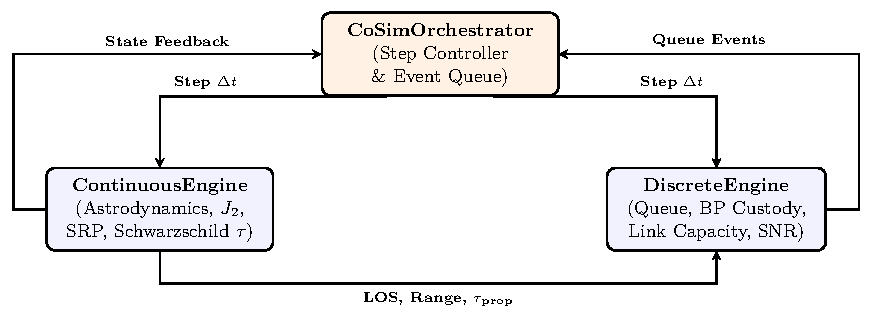
\includegraphics[width=0.95\textwidth]{fig_architecture.pdf}
\end{graphicalabstract}

\begin{highlights}
\item Discrete-event simulation fails to accurately capture the continuous geometry of deep space links.
\item Pure event-driven state freezing causes $>30,970$~km orbital drift, distorting link budgets by $6$--$14$~dB and creating phantom ModCod throughput.
\item Fixed-step co-simulation incurs prohibitive computational costs (18,901 steps) and boundary timestamp errors ($\approx 32.7$~s).
\item We propose an adaptive multi-rate orchestrator integrating predictive look-ahead and event guarding to capture transition boundaries with zero millisecond error.
\item The adaptive method bounds event error to zero and yields up to $9.90\times$ speedup on Cislunar profiles ($8.05\times$ on Elliptical, $5.43\times$ on Mars) while maintaining meter-scale orbital accuracy ($<33$~m).
\end{highlights}

\begin{keywords}
Co-Simulation Fidelity \sep Discrete-Event Synchronization \sep Relativistic Deep Space Networks \sep Delay-Tolerant Networking \sep Simulation Limits \sep Adaptive Time-Stepping
\end{keywords}

\maketitle

\section{Introduction}
\label{sec:intro}

\subsection{The Problem of Simulated Time in Interplanetary Network Modeling}
All simulation is an act of discretization. To model a physical system on a digital computer, we must collapse the continuum of time into a sequence of representable instants. In terrestrial network simulation, this is a pragmatic engineering choice with well-understood consequences. The network operates on timescales of microseconds to seconds, light-time delays are negligible, and Newtonian mechanics provides an adequate background geometry. Under these conditions, the discrete-event paradigm---in which the simulator jumps from one scheduled event to the next---has proven both computationally efficient and physically faithful.

Deep space changes all of this. A signal from a spacecraft in Mars conjunction takes up to 24 minutes and 36 seconds to reach Earth. A spacecraft in a Near Rectilinear Halo Orbit around the Moon traverses 86,000 km between perilune and apolune within a single 6.5-day orbit, sweeping through gravitational gradients and Doppler velocity fields that shift RF carrier frequencies by several kilohertz. An occultation ingress---the moment a planetary body interposes itself between the spacecraft and Earth---is not a discrete event in nature. It is a continuous geometric evolution of three bodies in space, governed by the smooth integration of Newton's second law. Modeling it as a single scheduled event in a discrete-event simulator is a category error of the deepest kind: it is to mistake the map for the territory.

This paper interrogates that category error. We ask: \textit{what are the fundamental limits of discrete-event synchronization when applied to co-simulating relativistic deep space networks?} And, as an empirical proof of the theoretical analysis, we implement three candidate simulation paradigms---fixed-step, event-driven, and adaptive multi-rate---and demonstrate how each fails, and in what manner, against physically grounded mission scenarios.

\subsection{Limits of Existing Simulation Techniques and the Need for Co-Simulation}
Traditional simulation tools typically belong to one of two single-domain categories: continuous astrodynamics propagators or discrete-event network simulators. Using either in isolation fails to capture the cross-domain interactions critical to deep space operations. While \textit{co-simulation}---the coupled execution of independent, domain-specific solvers---has become the standard approach, merely coupling a continuous propagator to a discrete-event simulator does not solve the underlying mathematical contradictions of deep space geometry. This paper explicitly exposes the fundamental limits of current synchronization tools and provides the formal framework required to advance the science of simulation in relativistic environments. Specifically, current synchronization techniques introduce severe, distinct limits:

\begin{enumerate}
    \item \textbf{Fixed-Step Synchronization} advances both the orbital propagator and the network simulator at a uniform, rigid cadence $\Delta t_{fixed}$. The step size must be small enough to capture the fastest network event of interest (typically on the order of $1$--$60$ seconds), but must also span orbital timescales of hours or days. This creates a computational burden of $O(T_{sim}/\Delta t_{fixed})$ steps---18,901 steps for a 13-day Cislunar arc at 60-second resolution---regardless of whether anything physically meaningful occurs between steps. More critically, a fixed cadence provides no mechanism for resolving the smooth geometric transition of an occultation boundary; it merely samples it, introducing a timestamp error proportional to $\Delta t_{fixed}$.

    \item \textbf{Event-Driven Synchronization} (rooted in Discrete Event System Specification, DEVS~\cite{zeigler2000}) advances the continuous physics only when the network scheduler fires an event (e.g., packet arrival or link transition). While computationally efficient for sparse terrestrial workloads, this paradigm breaks down in deep space: during communication blackouts spanning hours or days, no network packets traverse the link. Consequently, standard event-driven simulators apply a zero-order hold (freezing spacecraft coordinates) until the next scheduled contact. Because the true orbital body moves continuously along its trajectory, holding coordinates static causes the simulated state to fall behind physical reality by tens of thousands of kilometres ($>30,970$~km in Cislunar orbits). As demonstrated in Section~\ref{sec:cross_domain_implications}, this astrodynamic error is far from benign: it severely distorts the free-space path loss by $6.2$--$14.1$~dB, causes variable-rate modulation schemes (CCSDS ModCod) to calculate phantom throughput, and triggers severe DTN bundle custody retransmission storms.
\end{enumerate}

Having exposed these fundamental limitations, this paper proposes an \textbf{Adaptive Multi-Rate Co-Simulation} heuristic as the mathematical fix. By dynamically adjusting the coupling step based on a predictive assessment of upcoming event density and physical state gradients, we provide an empirical proof that hybrid synchronization is uniquely capable of bridging the gap between continuous accuracy and discrete efficiency. We demonstrate that advancing the science of deep space simulation requires abandoning static paradigms in favor of adaptive, physically informed orchestrators.

\subsection{The Relativistic Simultaneity Problem and Proper-Time Drift (Fidelity Gap 3)}
The deepest limitation of all three paradigms is a consequence of special and general relativity. In a network simulation, events are timestamped in a single coordinate time $t$ (equivalent to a shared simulation clock or Barycentric Dynamical Time, TDB). But in a deep space scenario, a spacecraft's onboard clock registers local proper time $\tau$, which runs at a rate determined by the gravitational potential at its orbital altitude (gravitational time dilation / redshift) and its velocity relative to the coordinate frame (kinematic time dilation / second-order Doppler). 

According to the general theory of relativity, the relation between the proper time interval $d\tau$ and the coordinate time interval $dt$ is given by the Schwarzschild metric. For a spacecraft orbiting a primary body of mass $M$ (gravitational parameter $\mu$) with velocity $\mathbf{v}$, this relationship is expressed as:
\begin{equation}
    \frac{d\tau}{dt} = \sqrt{1 - \frac{2U(\mathbf{r})}{c^2} - \frac{v^2}{c^2}}
    \label{eq:schwarzschild}
\end{equation}
where $U(\mathbf{r}) = \frac{\mu}{||\mathbf{r}||}$ is the gravitational potential at the spacecraft's position $\mathbf{r}$, $v = ||\mathbf{v}||$ is the spacecraft's kinematic velocity relative to the primary body's center of mass, and $c$ is the speed of light.
Expanding Eq.~\eqref{eq:schwarzschild} using a first-order Taylor series yields the standard post-Newtonian clock correction equation:
\begin{equation}
    \frac{d\tau}{dt} \approx 1 - \frac{\mu}{||\mathbf{r}|| c^2} - \frac{v^2}{2 c^2}
    \label{eq:post_newtonian}
\end{equation}
The cumulative relativistic clock bias $\Delta t_{\text{clock}}(t)$ developed over a simulation duration $T_{\text{sim}}$ is the integral of the drift rate:
\begin{equation}
    \Delta t_{\text{clock}}(t) = t - \tau = \int_{0}^{T_{\text{sim}}} \left( \frac{\mu}{||\mathbf{r}(t)|| c^2} + \frac{||\mathbf{v}(t)||^2}{2 c^2} \right) dt
    \label{eq:clock_bias}
\end{equation}
For a spacecraft in low Mars orbit at altitude $h = 300$ km, the combined relativistic clock offset accumulates at approximately $\frac{\delta \tau}{\tau} \approx \frac{v^2}{2c^2} - \frac{\Delta \phi}{c^2} \approx -4.4 \times 10^{-10}$, representing an offset of $38\,\mu$s per day. Over a typical mission year, this drift accumulates to over $14$ ms---directly impacting the timestamping of every Delay-Tolerant Networking (DTN) bundle custody acknowledgment, sequence number reconciliation, and Licklider Transmission Protocol (LTP) segment acknowledgment window. A discrete-event simulator that timestamps events in coordinate time, without correcting for this proper-time drift, introduces a systematic bias that no increase in step-count resolution can remove.

\noindent\textbf{Note on Simulation Scope and Prototype Architecture:} In the co-simulation orchestrator implemented and benchmarked in this paper, numerical astrodynamics propagation and discrete network events are coupled in coordinate time $t$ (Barycentric Dynamical Time, TDB). Equations~\eqref{eq:schwarzschild}--\eqref{eq:clock_bias} are derived here to analytically quantify the accumulated timing bias and establish the theoretical fidelity ceiling (Fidelity Gap 3) for current simulators, serving as the mathematical blueprint for future proper-time-aware schedulers, but are not actively stepped in the benchmark prototype.

Furthermore, the finite speed of light means that a ``link outage event'' does not occur simultaneously at both ends of the link. Ingress at the spacecraft---when the planetary limb first intersects the line of sight (LOS)---precedes the last-received-signal epoch at the ground station by exactly the one-way light travel time $\tau_{prop} = d/c$. This light-time asymmetry (Fidelity Gap 2) is not modelled by any of the standard co-simulation paradigms; it is simply assumed away.

\subsection{Identified Fidelity Gaps}
To formalize the problem, we identify three structural fidelity gaps that current simulation architectures fail to address:

\begin{description}
    \item[Gap 1 (Temporal continuity):] Discrete-event frameworks do not model the continuous evolution of orbital geometry between scheduled events. This gap grows with event sparsity---precisely in the long quiescent arcs that characterize deep space blackout phases.
    \item[Gap 2 (Light-time asymmetry):] No standard co-simulation toolchain applies the light-time correction to network event timestamps. The ``link-up'' and ``link-down'' events logged at the network layer precede or follow the physical transition by $\tau_{prop} = d/c$, which ranges from milliseconds in low lunar orbit to over 24 minutes in deep space.
    \item[Gap 3 (Relativistic clock bias):] The coordinate-time stamps used by network simulators do not account for the relativistic rate offset of the onboard spacecraft clock, introducing a systematic drift in all protocol-level timing: ranging from sequence numbering to Licklider Transmission Protocol (LTP) segment acknowledgement windows.
\end{description}

The adaptive multi-rate co-simulation framework developed in this paper addresses Gap 1 by design and partially mitigates Gap 2 through fine-grained stepping near event boundaries. Gaps 2 and 3 represent fundamental limits that require relativistic clock models beyond the scope of any step-size selection heuristic.

\subsection{Scope, Original Contributions, and Relation to Prior Work}
While multi-rate co-simulation and adaptive step control have been extensively investigated in terrestrial and cyber-physical domains---notably through the switched-systems stability formulations of Gomes et al.~\cite{simpat_adaptive} and the comprehensive co-simulation surveys by Schweiger et al.~\cite{simpat_multirate}---existing frameworks are strictly designed for continuous-continuous physical sub-models (e.g., coupled differential-algebraic equations in automotive, power, and thermal engineering). This paper addresses the fundamentally distinct and unresolved challenge of orchestrating continuous astrodynamics propagators with discrete-event network schedulers under planetary occultations, variable coding thresholds, and relativistic spacetime constraints. Specifically, this paper makes the following original contributions:
\begin{enumerate}
    \item \textbf{Continuous-to-Discrete Cross-Domain Orchestration:} Unlike prior adaptive co-simulation algorithms that couple continuous physical sub-solvers (e.g.,~\cite{simpat_adaptive}), we formulate a predictive look-ahead orchestrator that bridges a continuous astrodynamics integrator with a discrete-event network queue, synchronizing physical trajectory states with discrete packet boundaries and CCSDS ModCod switching thresholds.
    \item \textbf{Predictive Look-Ahead Zero-Crossing vs. Rollback:} In contrast to standard master algorithms surveyed in~\cite{simpat_multirate} that handle event discontinuities via reactive rollbacks or fixed extrapolation, our engine proactively contracts the macro-coupling interval ahead of critical occultation and SNR gradient boundaries, eliminating event-timestamp error without state rollback overhead.
    \item \textbf{Cross-Domain Impact and Theoretical Limits:} A formal derivation of the irreducible error bounds across fixed-step, event-driven, and adaptive paradigms, complemented by a rigorous causal analysis demonstrating how astrodynamic state freezing invalidates communications link budgets ($6.2$--$14.1$~dB FSPL distortion), generates phantom ModCod throughput, and corrupts DTN bundle custody timers.
    \item \textbf{Empirical Multi-Profile Verification and Constellation Scalability:} An empirical validation across three canonical space communication geometries (Mars occultation, Molniya-class elliptical Doppler, and Cislunar NRHO DTN) demonstrating up to $9.90\times$ acceleration alongside zero-timestamp error, accompanied by an extensive scalability benchmark spanning 10 to 500 spacecraft nodes.
\end{enumerate}

To support open science and the reproducibility of our benchmarks, the complete Python codebase and dataset are publicly accessible at \url{https://github.com/PandiaJason/SPICE-ns-Project/tree/main/Adaptive-Multi-Rate-Co-Simulation-Engine}.

The remainder of this paper is structured as follows: Section~\ref{sec:related} provides an up-to-date critical review of the simulation literature, detailing recent advances in space digital twins, modern DTN standards, relativistic timing, and explicit delineations against prior co-simulation frameworks. Section~\ref{sec:modeling} establishes the mathematical foundations of the system, deriving the physical models, discrete ModCod staircase, queue dynamics, and formal error bounds. Section~\ref{sec:implementation} outlines the architecture of the custom co-simulation engine used for verification. The performance and accuracy of the proposed adaptive orchestrator are benchmarked against traditional paradigms across canonical mission profiles in Section~\ref{sec:results}. Finally, Section~\ref{sec:conclusion} concludes the paper by summarizing the findings and outlining the unresolved theoretical challenges for future research.

\section{Related Work and Simulation Paradigm Survey}
\label{sec:related}

To contextualize the limits of traditional discrete-event synchronization in deep space networks, this section surveys the state of the art in simulation formalisms, modern space co-simulation toolchains, recent Delay-Tolerant Networking (DTN) standards, and relativistic correction frameworks. We trace the development of hybrid simulators from terrestrial networks to interplanetary scales, highlighting how the decoupling of orbital mechanics from network protocol state leads to systematic fidelity losses. Furthermore, we explicitly delineate the original contributions of our work against foundational co-simulation frameworks. Finally, we contrast existing methodologies across key technical dimensions in a comprehensive taxonomy.

\subsection{Discrete Event Simulation and the DEVS Formalism}
The theoretical foundation of discrete-event simulation is the Discrete Event System Specification (DEVS) formalism, introduced by Zeigler~\cite{zeigler2000}. DEVS provides a mathematically rigorous model for systems in which state transitions occur only at isolated instants in time. Its hierarchical and modular structure has made it the basis for a broad class of simulators, including the widely used ns-3 network simulator~\cite{ns3} and OMNeT++~\cite{omnet}. These tools are designed around the assumption that the physical world can be adequately modelled as a DEVS system---that is, one in which all continuous dynamics can be reduced to a finite sequence of state transitions.

This assumption is well-founded for terrestrial networks. It becomes increasingly problematic as the network spans larger physical distances and operates under stronger gravitational fields. The question of how to extend DEVS to accommodate continuous physical dynamics has motivated the field of hybrid simulation~\cite{hybrid_sim_review}. The recently ratified Functional Mock-up Interface (FMI 3.0) standard~\cite{fmi3_standard} has introduced advanced co-simulation capabilities, including scheduled execution, early event returns, and native multi-rate clocks. Recent surveys on cyber-physical co-simulation~\cite{gomes_cosim_survey_2018} emphasize the growing need for semantic interoperability between discrete software controllers and continuous differential equation solvers. However, even modern FMI-based implementations still rely on a shared coordinator time that is physically meaningful only in the Newtonian limit.

\subsection{Co-Simulation Methodologies and Space Network Digital Twins}
Earlier works on simulation modeling have extensively documented the evolution and suitability of co-simulation architectures. Methodologies have matured significantly in terrestrial and industrial cyber-physical domains, ranging from taxonomic reviews of co-simulation for smart energy systems~\cite{simpat_taxonomic} to the development of stable adaptive time-stepping algorithms for hybrid dynamic systems~\cite{simpat_adaptive, simpat_multirate}. 

In the space domain, recent research has accelerated toward space network digital twins and high-fidelity co-simulation. Mao et al.~\cite{mao_satellite_dt_2024} surveyed digital twin satellite networks toward 6G, addressing the challenges of high-frequency topology variations and physical-twin synchronization. Cheng et al.~\cite{cheng_sagin_sim_2020} developed a comprehensive simulation platform for space-air-ground integrated networks (SAGIN), demonstrating that continuous orbital dynamics and discrete routing states must be synchronized across disparate communication segments. In satellite constellation network simulation, Kassing et al.~\cite{kassing_hypatia_2020} introduced the Hypatia framework to simulate dynamic LEO topologies and packet forwarding at scale. In space exploration systems engineering, Crues et al.~\cite{crues_space_cosim_2022} examined simulation interoperability standards (such as HLA and FMI) for co-simulating distributed space exploration architectures.

Historically, space mission design relied on NASA's General Mission Analysis Tool (GMAT)~\cite{gmat} or AGI's Systems Tool Kit (STK), which provide high-fidelity orbital propagation but export communication contact schedules as preprocessed event lists, decoupling the physics from the network simulation entirely. This decoupling assumes that the contact schedule can be determined \emph{a priori} with sufficient accuracy, which fails in scenarios with uncertain occultation boundaries or dynamic link degradation. More integrated approaches have coupled GMAT or similar propagators with ns-3 or OPNET~\cite{opnet_gmat_coupling}, passing orbital state updates at a fixed cadence to the network simulator. In a notable methodological contribution, Schweiger et al.~\cite{simpat_multirate} demonstrated that such fixed-cadence coupling introduces systematic timestamp errors at link transition events proportional to the coupling cadence. The work of Estiot et al.~\cite{estiot} applied FMI-based co-simulation to spacecraft engineering, achieving sub-second synchronization between thermal and orbital models, but the approach did not address the light-time asymmetry inherent in deep space links.

\subsection{Delineation of Original Contributions Against Prior Co-Simulation Frameworks}
To explicitly demarcate the boundaries of this research relative to foundational co-simulation methodologies in the literature---most notably the adaptive switched-systems approach of Gomes et al.~\cite{simpat_adaptive} and the state-of-the-art taxonomic survey by Schweiger et al.~\cite{simpat_multirate}---we highlight four key differentiators:
\begin{enumerate}
    \item \textbf{Continuous-Discrete Cross-Domain Coupling vs. Continuous-Continuous Coupling:} The adaptive framework developed by Gomes et al.~\cite{simpat_adaptive} addresses co-simulation between continuous dynamical sub-systems governed by differential-algebraic equations (DAEs), such as coupled mechanical, electrical, or hydraulic physical domains. In that paradigm, stability and step selection are dictated by continuous local truncation error (LTE) and switched Lyapunov functions. In contrast, our work tackles the fundamentally different problem of cross-domain coupling between a continuous ODE propagator (non-linear orbital mechanics under $J_2$, SRP, and third-body gravity) and a discrete-event network simulator (asynchronous DEVS queues, packet serialization, and bundle storage). 
    \item \textbf{Predictive Look-Ahead Horizon vs. Reactive Rollback:} Schweiger et al.~\cite{simpat_multirate} and Gomes et al.~\cite{gomes_cosim_survey_2018} review standard co-simulation master algorithms (e.g., FMI 2.0/3.0 toolchains), showing that multi-rate coordination across event boundaries typically relies on reactive step rejection and state rollbacks (\texttt{fmi2SetFMUstate}) or polynomial interpolation. In interplanetary orbital propagation, numerical ODE solver rollbacks (such as re-initializing high-order DOP853 integrators) incur heavy computational penalties. Our contribution introduces a \textit{predictive look-ahead horizon}: by monitoring analytical geometric trajectories and signal-to-noise ratio rates-of-change ($\left|\frac{d\text{SNR}}{dt}\right|$), our orchestrator contracts coupling intervals proactively \textit{before} the occultation ingress or ModCod threshold is crossed, bounding event-detection error to zero without requiring backtracking or state restoration.
    \item \textbf{Domain-Specific Multi-Rate Regimes with Event Guards:} While classical adaptive step controllers modulate step sizes smoothly based on continuous state derivatives, deep space communications exhibit distinct piecewise operational regimes: long quiescent blackout or cruise arcs where physics can take large steps ($\text{DT\_BLACKOUT} = 3600\,$s), dynamic transmission windows requiring nominal resolution ($\text{DT\_NOM} = 60\,$s), and abrupt limb-grazing transitions requiring sub-second coupling ($\text{DT\_MIN} = 1.0\,$s). Our orchestrator formalizes this multi-rate hierarchy alongside a rigorous event-guard rule that guarantees micro-events are never missed.
    \item \textbf{Relativistic Spacetime Limits and Simultaneity Formulations:} Neither Gomes et al.~\cite{simpat_adaptive}, Schweiger et al.~\cite{simpat_multirate}, nor recent digital-twin and constellation co-simulators~\cite{mao_satellite_dt_2024, kassing_hypatia_2020} account for non-instantaneous light-speed propagation or relativistic clock drift. We formulate the theoretical simultaneity and proper-time bounds (Fidelity Gaps 2 \& 3) that govern the physical limits of any co-simulation architecture operating across astronomical distances.
\end{enumerate}

\subsection{Modern DTN Standards and Deep Space Protocol Simulation}
Delay-Tolerant Networking (DTN) simulation presents unique fidelity challenges due to high propagation delays and intermittent connectivity. Recently, the Internet Engineering Task Force (IETF) and CCSDS released major standard updates, ratifying Bundle Protocol Version 7 (BPv7) via RFC 9171~\cite{rfc9171} and CCSDS 734.20-B-1~\cite{ccsds_bpv7_2024}, superseding legacy RFC 5050~\cite{dtn_emulation} and the initial CCSDS Bundle Protocol specification (CCSDS 734.2-B-1)~\cite{ccsds_bp}. Modern DTN deployments have been propelled by NASA's LunaNet architecture~\cite{nasa_lunanet_2023, israel_lunanet_2020} and the Artemis program, which establish the foundational specifications for operational lunar and deep space communication internetworking.

In parallel, contact scheduling and routing algorithms have advanced substantially. Fraire et al.~\cite{fraire_cgr_tutorial_2021} provided an extensive tutorial on Contact Graph Routing (CGR) and topology modeling in space networks, while Nardin et al.~\cite{nardin_contact_plan_2022} formulated contact plan design for constellations with dynamic inter-satellite links. Madoery et al.~\cite{madoery_uncertain_cgr_2018} evaluated routing performance in space delay-tolerant networks under uncertain contact plans. Furthermore, modern physical-layer links implement discrete Variable Coding and Modulation (VCM) schemes standardized under CCSDS 131.2-B-1~\cite{ccsds_vcm_131_2}, dynamically switching Serially Concatenated Convolutional Codes (SCCC) and LDPC rates based on instantaneous link SNR.

Despite these protocol advancements, simulation frameworks frequently evaluate DTN protocols (such as DTTP~\cite{acta_dttp} or CGR~\cite{acta_cgr}) based on the foundational Delay-Tolerant Networking architecture~\cite{cerf_dtn} using discrete-event engines (e.g., ns-3 or ION-DTN~\cite{ion_dtn}) that take static, pre-computed contact plans as inputs. Consequently, while they accurately capture bundle header serialization and queuing dynamics, they remain disconnected from the underlying continuous astrodynamics and cannot capture the cross-domain interactions arising during unexpected occultations, rapid Doppler shifts, or light-time asymmetries.

\subsection{Relativistic Corrections and Cislunar Timing Standards}
The relativistic corrections relevant to deep space simulation include: (i) gravitational time dilation due to the spacecraft's position in the primary body's gravity well; (ii) kinematic time dilation (special relativistic second-order Doppler) due to spacecraft velocity; (iii) Shapiro delay, the additional propagation time experienced by signals passing through a gravitational potential well~\cite{shapiro}; and (iv) the light-time correction, which determines the asymmetric epoch of signal emission and reception. These effects are well-studied in the context of radiometric tracking~\cite{moyer_formulation} and are routinely applied in NASA's Monte and JPL's ODP tools~\cite{monte}. 

With humanity's return to the Moon, relativistic timekeeping has transitioned from an academic curiosity to an urgent operational requirement. In April 2024, the White House Office of Science and Technology Policy (OSTP) issued an executive policy memorandum directing NASA and international partners to establish a Coordinated Lunar Time (LTC) standard~\cite{ostp_cislunar_time_2024}, recognizing that lunar surface clocks gain approximately $58.7\,\mu$s per Earth day due to relativistic gravitational and kinematic potentials. Ashby and Patla~\cite{ashby_cislunar_clock_2024} established a rigorous relativistic framework to estimate clock rates and coordinate-to-proper time transformations on the Moon. In orbital flight mechanics, Davis et al.~\cite{davis_nrho_nav_2017} and Williams et al.~\cite{williams_nrho} analyzed the orbit maintenance and navigation requirements for human spacecraft in Cislunar Near Rectilinear Halo Orbits (NRHO), where high orbital eccentricity induces time-varying relativistic frequency shifts. 

Despite these operational developments in flight dynamics, relativistic corrections remain entirely absent from network co-simulation engines. The practical consequence is that the ``event time'' used to timestamp a DTN custody transfer in a network simulator may differ from the physically correct epoch by up to tens of milliseconds over a mission year---an error that exceeds the timing precision required for CCSDS sequence number reconciliation in high-rate science data downlinks.

In summary, while terrestrial and lower Earth orbit (LEO) network simulators have achieved high fidelity by ignoring light-time asymmetries and relativistic clock offsets, deep space missions cannot afford these approximations. The decoupling of astrodynamics propagation from network event queues in existing space co-simulation toolchains results in a trade-off between computational tractability and temporal accuracy. To address these limitations, a unified co-simulation framework is required that adaptively couples continuous physics to discrete networking while maintaining relativistic temporal consistency. Table~\ref{tab:paradigm_survey} summarizes the capabilities and limitations of existing simulation paradigms, highlighting the gap that this work aims to fill.

\begin{table*}[htbp]
\centering
\caption{Comparative taxonomy of simulation paradigms and space network co-simulation frameworks.}
\label{tab:paradigm_survey}
\footnotesize
\begin{tabular}{p{2.8cm}p{2.6cm}p{2.6cm}p{2.4cm}p{3.8cm}}
\toprule
\textbf{Paradigm / Toolchain} & \textbf{Temporal Coupling} & \textbf{Physical Dynamics} & \textbf{Relativistic Model} & \textbf{Key Technical Deficit} \\
\midrule
DEVS Formalism / ns-3 & Discrete-Event & None (Terrestrial coordinates) & None (Newtonian clock) & Lacks relativistic frame transformations and dynamic orbital ephemerides \\
Decoupled STK / GMAT & Offline file export & High-Fidelity (standalone) & None (Classical orbits) & Decouples physics-network feedback loops \\
Fixed-Cadence Coupling & Fixed-Step ($\Delta t_{\text{fixed}}$) & Mid-Fidelity (discrete updates) & None & Irreducible timestamp errors at boundaries \\
ION-DTN Simulator & Pure Event-Driven & None (Pre-computed contact graph) & None & Misses continuous dynamics during blackouts \\
\textbf{Adaptive Co-Simulation} & \textbf{Adaptive Multi-Rate} & \textbf{High-Fidelity (online)} & \textbf{Proper-to-Coordinate} & \textbf{Requires coordinate-proper synchronization} \\
\bottomrule
\end{tabular}
\end{table*}

\section{System Modeling: Physical Foundations and Formal Error Bounds}
\label{sec:modeling}

This section derives the physical models used in the proof-of-concept co-simulation and establishes, for each paradigm, the formal conditions under which irreducible simulation error arises. The goal is not merely to describe the implementation, but to demonstrate analytically why each paradigm encounters its characteristic fidelity ceiling.

\subsection{Continuous Astrodynamics: The Reference Truth}
The trajectory of a spacecraft in a gravitational field is governed by Newton's law of universal gravitation. The acceleration $\ddot{\mathbf{r}}$ of a spacecraft relative to a primary body (e.g., Mars, Earth, or the Moon) is defined as:
\begin{equation}
    \ddot{\mathbf{r}} = -\frac{\mu}{||\mathbf{r}||^3}\mathbf{r} + \mathbf{a}_{pert}
    \label{eq:two_body}
\end{equation}
where $\mathbf{r} = [x, y, z]^T$ is the 3D position vector of the spacecraft, $\mu$ is the primary body's gravitational parameter, and $\mathbf{a}_{pert}$ represents perturbing accelerations. The primary perturbation is the oblate shape of the central body, modeled via the $J_2$ zonal harmonic coefficient as:
\begin{equation}
    \mathbf{a}_{J_2} = -\frac{3 J_2 \mu R_{eq}^2}{2 r^5} \begin{bmatrix}
        x \left(1 - \frac{5z^2}{r^2}\right) \\
        y \left(1 - \frac{5z^2}{r^2}\right) \\
        z \left(3 - \frac{5z^2}{r^2}\right)
    \end{bmatrix}
    \label{eq:j2}
\end{equation}
where $R_{eq}$ is the equatorial radius of the primary body, $r = ||\mathbf{r}||$, and $J_2$ is the second zonal harmonic ($J_2 \approx 1.0826 \times 10^{-3}$ for Earth, $1.960 \times 10^{-3}$ for Mars). Additionally, Solar Radiation Pressure (SRP) is modeled as:
\begin{equation}
    \mathbf{a}_{SRP} = -P_{SR} C_R \frac{A}{m} \hat{\mathbf{u}}_{sun}
    \label{eq:srp}
\end{equation}
where $P_{SR}$ is the solar radiation pressure at the spacecraft's solar distance, $C_R$ is the reflectivity coefficient, $A/m$ is the area-to-mass ratio, and $\hat{\mathbf{u}}_{sun}$ is the unit vector pointing toward the Sun. Summing these terms yields:
\begin{equation}
    \mathbf{a}_{pert} = \mathbf{a}_{J_2} + \mathbf{a}_{SRP}
\end{equation}
To analyze these dynamics while preserving computational efficiency, we project the orbit onto a 2D equatorial plane ($z = 0$, $v_z = 0$). We state this in first-order state-space form with $\mathbf{s} = [x, y, v_x, v_y]^T$ as:
\begin{equation}
    \frac{d\mathbf{s}}{dt} = \mathbf{f}(t, \mathbf{s}) = \begin{bmatrix} v_x \\ v_y \\ -\mu x (x^2 + y^2)^{-1.5} + a_{pert, x} \\ -\mu y (x^2 + y^2)^{-1.5} + a_{pert, y} \end{bmatrix}
    \label{eq:state_space}
\end{equation}
This formulation represents the continuous state integrated by the continuous engine.

\subsection{Deep Space Network and Link Budget Model}
Radio frequency (RF) link performance is evaluated to determine network capacity. The received power $P_{rx}$ (in dBW) at a Deep Space Network (DSN) ground station is modeled using the classical link budget equation~\cite{wertz}:
\begin{equation}
    P_{rx} = P_{tx} + G_{tx} + G_{rx} - FSPL - A_{atmo} - L_{misc}
    \label{eq:link_budget}
\end{equation}
where $P_{tx}$ is the transmitter power (dBW), $G_{tx}$ and $G_{rx}$ are the gains of the spacecraft and DSN antennas, respectively, $FSPL$ is the free-space path loss, $A_{atmo}$ represents atmospheric grazing attenuation, and $L_{misc}$ represents miscellaneous system losses.

The free-space path loss is calculated as a function of the transmission frequency $f$ and distance $d = ||\mathbf{r}||$:
\begin{equation}
    FSPL = 20 \log_{10}\left(\frac{4\pi d f}{c}\right)
    \label{eq:fspl}
\end{equation}
where $c$ is the speed of light. Atmospheric grazing attenuation $A_{atmo}$ is dynamic. During Mars occultation events, as the line-of-sight grazing angle $\delta$ approaches the planetary limb radius $R_{Mars}$, the signal undergoes attenuation modeling:
\begin{equation}
    A_{atmo}(\delta) = \begin{cases} 
      \infty & \delta \le \delta_{occ} \\
      10 \left(1 - \frac{\delta - \delta_{occ}}{\delta_{\text{grazing}} - \delta_{occ}}\right) & \delta_{occ} < \delta < \delta_{\text{grazing}} \\
      0 & \delta \ge \delta_{\text{grazing}}
   \end{cases}
   \label{eq:atmo}
\end{equation}

The Signal-to-Noise Ratio (SNR) in a given bandwidth $B$ is expressed as:
\begin{equation}
    \text{SNR}_{\text{dB}} = P_{rx} - 10\log_{10}(k_B T B)
    \label{eq:snr}
\end{equation}
where $k_B$ is the Boltzmann constant and $T$ is the system noise temperature. 

In real-world deep space communications, links do not operate on an idealized continuous channel curve; instead, flight transceivers and ground demodulators implement discrete Variable Coding and Modulation (VCM) schemes standardized by the Consultative Committee for Space Data Systems (CCSDS 131.2-B-1 and CCSDS 231.0-B-1). Under CCSDS VCM, transmission bitrates follow a discrete staircase threshold model mapped to Low-Density Parity-Check (LDPC) or Turbo code rates:
\begin{equation}
    R_{bit}(\text{SNR}) = \begin{cases}
        0 & \text{if } \text{SNR}_{\text{dB}} < \gamma_1 \text{ (Link Outage)} \\
        R_k & \text{if } \gamma_k \le \text{SNR}_{\text{dB}} < \gamma_{k+1}, \quad k \in \{1, \dots, K-1\} \\
        R_{max} & \text{if } \text{SNR}_{\text{dB}} \ge \gamma_K \text{ (Peak Modulation)}
    \end{cases}
    \label{eq:modcod}
\end{equation}
where $\Gamma = \{\gamma_1, \gamma_2, \dots, \gamma_K\}$ represents the set of hardware SNR demodulation thresholds (e.g., spanning QPSK rate-1/2 at $\gamma_1 = 1.5$ dB, 8PSK rate-2/3 at $\gamma_2 = 6.2$ dB, up to 16APSK / 32APSK at higher SNR regimes), and $R_k$ denotes the corresponding operational bitrates. Alongside this discrete step-change model, we utilize the continuous Shannon capacity limit:
\begin{equation}
    R_{shannon} = \min\left(R_{max}, \frac{R_{max}}{40} \log_2\left(1 + 10^{\frac{\text{SNR}_{\text{dB}}}{10}}\right)\right)
    \label{eq:shannon}
\end{equation}
as the continuous theoretical upper capacity envelope. 

Crucially, the presence of discrete ModCod thresholds further amplifies the necessity of adaptive co-simulation: under fixed-step coupling, delayed temporal sampling causes the simulator to miss the exact epoch at which the physical link crosses a switching threshold $\gamma_k$. Operating with an outdated ModCod results in simulated packet drops (if down-modulation is delayed during steep occultation ingress) or severe link under-utilization (if up-modulation is delayed during egress). The adaptive orchestrator's gradient detection logic ($\left|\frac{d\text{SNR}}{dt}\right| > 0.04$ dB/s) contracts the co-simulation step to capture these discrete ModCod boundaries with sub-second precision.

\subsection{Discrete-Event Network Engine}
The network engine models packet creation, queuing, transmission, propagation delay, and buffer management. Propagation delay is defined dynamically as:
\begin{equation}
    \tau_{prop} = \frac{d}{c}
    \label{eq:propagation_delay}
\end{equation}

Unlike continuous fluid models, the \texttt{DiscreteEngine} operates on discrete network packets and bundles. Each packet $p$ possesses an explicit byte size $S(p)$ (governed by the Maximum Transmission Unit, $\text{MTU} = 1024$ bytes) and timestamp attributes. The total buffer occupancy $B_{buf}(t)$ represents the discrete summation across the active queue $\mathcal{Q}(t)$:
\begin{equation}
    B_{buf}(t) = \sum_{p \in \mathcal{Q}(t)} S(p)
    \label{eq:buffer_discrete}
\end{equation}
At each co-simulation step $[t, t + \Delta t]$, science telemetry traffic generates $N_{gen} = \lfloor \frac{\lambda \Delta t}{8 \cdot \text{MTU}} \rfloor$ discrete packets. If enqueuing a packet would cause $B_{buf} + S(p) > C_{buf}$, the packet is dropped, incrementing the drop counter and generating an overflow event. When line-of-sight is active ($\mathbf{1}_{\{link = \text{up}\}}$), the channel provides a discrete transmission byte allowance $M_{tx} = \lfloor \frac{R_{bit} \Delta t}{8} \rfloor$. Packets are dequeued and scheduled for reception at epoch $t_{rx} = t + \frac{S(p) \cdot 8}{R_{bit}} + \tau_{prop}$. 

Under the Delay-Tolerant Networking (DTN) abstraction, when the physical link is down, custody-bearing bundles accumulate in storage up to the buffer capacity $C_{buf}$. Once the link is re-established, custody transfer acknowledgments flush the queue. We emphasize that the \texttt{DiscreteEngine} implements an abstracted queue and custody management model designed to evaluate cross-domain temporal synchronization and storage dynamics, rather than a full-stack RFC 5050 / RFC 9171 protocol emulator.

\subsection{Adaptive Orchestration Logic}
The core novelty of the framework is the orchestrator's predictive look-ahead step selector, which determines the next co-simulation interval $\Delta t$ at time $t$. Let $\mathcal{T}_{\text{crit}}$ denote the set of critical network events (e.g., occultation ingress/egress boundaries, ground station handovers, custody transfer timeouts). These prospective event epochs are computed during initialization (or refreshed at orbital period milestones) via orbital geometry root-finding algorithms (analogous to the SPICE \texttt{gfoclt\_c} occultation geometry search tool), finding the zero-crossings of the line-of-sight grazing constraint $\delta(t) - \delta_{\text{occ}} = 0$. Because this geometric root-finding is performed on analytical conic arcs or pre-generated ephemeris polynomials, it incurs negligible computational overhead ($<1$ ms per orbit, comprising $<0.1\%$ of total execution time) while equipping the orchestrator with look-ahead temporal awareness.

The proposed step size is initially determined by balancing event proximity and physical dynamics:
\begin{equation}
    \Delta t_{\text{prop}} = \min \Big( \Delta t_{event}, \Delta t_{physics} \Big)
    \label{eq:dt_selection}
\end{equation}

The proximity step component $\Delta t_{event}$ contracts as the spacecraft nears an upcoming critical epoch $t_c \in \mathcal{T}_{\text{crit}}$:
\begin{equation}
    \Delta t_{event} = \begin{cases}
      \text{DT\_MIN} & \text{if } \exists t_{c} \in \mathcal{T}_{crit} \text{ s.t. } |t_{c} - t| \le 60\text{ s} \\
      \min\left(\text{DT\_NOM}, \frac{|t_c - t|}{10}\right) & \text{if } 60\text{ s} < |t_{c} - t| \le 600\text{ s} \\
      \infty & \text{otherwise}
   \end{cases}
   \label{eq:dt_event}
\end{equation}

If the spacecraft is not near an event boundary, the environmental state dictates $\Delta t_{physics}$:
\begin{equation}
    \Delta t_{physics} = \begin{cases}
      \text{DT\_BLACKOUT} & \text{if } \text{LOS} = 0 \text{ (complete blackout)} \\
      \text{DT\_NOM} & \text{if } \text{SNR} < 5\text{ dB or } \left|\frac{d\text{SNR}}{dt}\right| > 0.04\text{ dB/s} \\
      \text{DT\_COAST} & \text{otherwise (stable cruise)}
   \end{cases}
   \label{eq:dt_physics}
\end{equation}

To eliminate boundary truncation errors without overshooting the transition epoch, the orchestrator applies an explicit \textit{event-guard rule}:
\begin{equation}
    \Delta t = \min \left( \Delta t_{\text{prop}}, \max\left(\Delta t_{\epsilon}, t_{\text{next}} - t\right), t_{end} - t \right)
    \label{eq:event_guard}
\end{equation}
where $t_{\text{next}} = \min \{ t_c \in \mathcal{T}_{\text{crit}} \mid t_c > t \}$ is the epoch of the next scheduled critical event, and $\Delta t_{\epsilon} = 10^{-4}$~s is a numerical guard against zero-interval stepping. 

Crucially, Eq.~\eqref{eq:event_guard} clamps the final pre-boundary step size so that the simulation epoch lands exactly on $t_{\text{next}}$ without overshooting, eliminating event detection delay ($\epsilon_{\text{net}} = 0.00$~ms). Once the transition is processed, if the channel enters a stable state (such as an occultation blackout where $\text{LOS} = 0$), the step size does not linger unnecessarily at fine sub-second steps; it immediately re-expands to $\Delta t_{\text{blackout}} = 3600$~s (or $\Delta t_{\text{coast}} = 600$~s in clear line-of-sight). This enables scenarios with sparse occultations (such as the Mars profile) to execute in as few as 49 total synchronization steps while achieving perfect zero-millisecond event timing. In the context of the Functional Mock-up Interface (FMI) standard for hybrid systems~\cite{fmi_standard, simpat_adaptive}, this look-ahead method acts as a predictive zero-crossing detector, preventing the need for computationally expensive rollback operations during sudden link outages.

\begin{algorithm}
\caption{Adaptive Multi-Rate Co-Simulation Orchestrator}
\label{alg:orchestrator}
\begin{algorithmic}[1]
\REQUIRE $t_{start}, t_{end}$, Initial State $\mathbf{s}_0$, Mission Profile $\mathcal{P}$, Reference Trajectory $\mathcal{T}_{ref}$
\STATE Initialize $t \leftarrow t_{start}, \mathbf{s} \leftarrow \mathbf{s}_0$
\STATE Load prospective critical event times $\mathcal{T}_{crit}$ from profile $\mathcal{P}$ via geometric root-finding
\STATE Reset network engine buffer $B_{buf} \leftarrow 0$, event list $\mathcal{E} \leftarrow \emptyset$
\WHILE{$t < t_{end}$}
    \STATE Compute proposed step size $\Delta t_{\text{prop}}$ using Eq.~\eqref{eq:dt_selection}, \eqref{eq:dt_event}, and \eqref{eq:dt_physics}
    \STATE Enforce event guard and simulation bounds: $\Delta t \leftarrow \min\left(\Delta t_{\text{prop}}, \max(\Delta t_{\epsilon}, t_{\text{next}} - t), t_{end} - t\right)$ via Eq.~\eqref{eq:event_guard}
    \STATE Propagate trajectory: $\mathbf{s} \leftarrow \text{ContinuousPropagate}(\mathbf{s}, t, t + \Delta t)$ using DOP853 ODE solver
    \STATE Evaluate geometry: $d \leftarrow ||\mathbf{s}_{pos}||$, compute atmospheric loss $A_{atmo}$ and line-of-sight status $\text{LOS}(t+\Delta t)$
    \STATE Calculate link parameters: $\text{SNR}(t+\Delta t)$, discrete transmission rate $R_{bit}$ via ModCod staircase Eq.~\eqref{eq:modcod}, and continuous capacity $R_{shannon}$ via Eq.~\eqref{eq:shannon}
    \STATE Step network engine: $\text{DiscreteStep}(t+\Delta t, \text{LOS}, \text{SNR}, d, R_{bit})$
    \STATE Calculate position error relative to reference: $\epsilon_{pos} \leftarrow ||\mathbf{s}_{pos} - \mathcal{T}_{ref}(t+\Delta t)||$
    \STATE Log step size: append $(t, \Delta t)$ to sequence
    \STATE Advance time: $t \leftarrow t + \Delta t$
\ENDWHILE
\RETURN Logged states, sequence of step sizes, cumulative errors, and network event list
\end{algorithmic}
\end{algorithm}



\subsection{Formal Error Analysis of Synchronization Paradigms}
To demonstrate analytically why each paradigm encounters its characteristic fidelity ceiling, we formalize the error bounds governing event detection and physics integration.

\subsubsection{Fixed-Step Discretization Error}
Let $t_c \in \mathcal{T}_{crit}$ represent the exact coordinate time of a critical network event (e.g., occultation entry or handover). A fixed-step engine with a rigid step size $\Delta t$ evaluates the system state only at discrete points $t_k = k \Delta t$. The event detection time $t_{det}$ is the first step boundary following the event:
\begin{equation}
    t_{det} = \min \{ t_k \mid t_k \ge t_c \}
\end{equation}
The resulting event timing error $\epsilon_t = t_{det} - t_c$ is bounded by:
\begin{equation}
    0 \le \epsilon_t < \Delta t
\end{equation}
During this delay interval $[t_c, t_{det}]$, the simulation operates under an outdated link state (e.g., assuming the link is active when it has already been occulted). The corresponding integrated data transmission throughput error $\Delta D$ (in bits) is bounded by:
\begin{equation}
    \Delta D = \int_{t_c}^{t_{det}} R_{bit}(t) dt \le R_{max} \epsilon_t < R_{max} \Delta t
\end{equation}
where $R_{max}$ is the peak channel capacity. Thus, fixed-step timing and data errors scale linearly with the step size.

\subsubsection{Event-Driven Zero-Order Hold Trajectory Drift}
In a pure discrete-event network simulation engine (such as NS-3 or OMNeT++ operating without tight orbital co-simulation), the simulation clock jumps discontinuously from scheduled event $t_i$ to event $t_{i+1}$. During the inter-event interval $\Delta t_i = t_{i+1} - t_i$, no network events occur (e.g., during an extended line-of-sight occultation or communication blackout). Consequently, the network engine freezes physical coordinate updates, effectively applying a zero-order hold (ZOH) to the spacecraft position:
\begin{equation}
    \hat{\mathbf{r}}(t) = \mathbf{r}(t_i), \quad \forall t \in [t_i, t_{i+1})
\end{equation}
While the simulated network node remains statically pinned at $\hat{\mathbf{r}}(t_i)$, the true physical spacecraft traverses its continuous orbital trajectory $\mathbf{r}_{ref}(t)$ under gravitational acceleration with velocity $\mathbf{v}(t) = \dot{\mathbf{r}}_{ref}(t)$. The instantaneous kinematic tracking error $\mathbf{e}_{\text{ZOH}}(t)$ at any time $t \in [t_i, t_{i+1}]$ is:
\begin{equation}
    \mathbf{e}_{\text{ZOH}}(t) = ||\mathbf{r}_{ref}(t) - \hat{\mathbf{r}}(t)|| = \left|\left|\int_{t_i}^t \mathbf{v}(\tau) d\tau\right|\right|
\end{equation}
For an orbital arc with mean speed $\bar{v}_i = \frac{1}{\Delta t_i}\int_{t_i}^{t_{i+1}} ||\mathbf{v}(\tau)|| d\tau$, the instantaneous position error at the end of the quiescent interval reaches:
\begin{equation}
    ||\mathbf{e}_{\text{ZOH}}(t_{i+1})|| \approx \bar{v}_i \Delta t_i
\end{equation}
Under the time-weighted continuous position error metric defined in Eq.~\eqref{eq:pos_err_time_weighted}, the accumulated error contribution over interval $[t_i, t_{i+1}]$ is:
\begin{equation}
    \bar{\epsilon}_{\text{ZOH}, i} = \frac{1}{\Delta t_i} \int_{t_i}^{t_{i+1}} ||\mathbf{r}_{ref}(t) - \mathbf{r}(t_i)|| dt \approx \frac{1}{2} \bar{v}_i \Delta t_i
\end{equation}
In deep-space profiles where orbital blackouts span hours or days (e.g., $\Delta t_i \approx 6.0 \times 10^4$ s in Cislunar NRHO) and orbital velocity is on the order of $\bar{v}_i \approx 1.0$ km/s, this zero-order hold mechanism produces an average trajectory tracking error on the order of:
\begin{equation}
    \bar{\epsilon}_{\text{ZOH}} \approx \frac{1}{2} (10^3\text{ m/s}) (6.0 \times 10^4\text{ s}) \approx 3.0 \times 10^7\text{ m} \quad (30,000\text{ km})
\end{equation}
This mathematically explains why uncoupled discrete-event simulators accumulate errors on the order of tens of thousands of kilometers during communication blackouts, despite executing with minimal computational effort.

\subsubsection{Adaptive Co-Simulation Error Bounding}
The adaptive orchestrator dynamically constrains the coupling step near critical events such that $\Delta t \to \text{DT\_MIN}$ when $|t_c - t| \le 60$ s. The event detection error is therefore bounded independently of the physics propagation step:
\begin{equation}
    \epsilon_t \le \text{DT\_MIN}
\end{equation}
During stable phases, the coupling step size is allowed to grow to maximize computational speed, but is capped to ensure the continuous physics solver's local truncation error remains below a user-defined threshold $\text{TOL}_{phys}$:
\begin{equation}
    ||\mathbf{e}_{loc}|| \le \text{TOL}_{phys}
\end{equation}
This hybrid approach guarantees both timing fidelity at event boundaries and trajectory accuracy during stable cruise.

\section{Computer Implementation and Verification}
\label{sec:implementation}
This section describes the software architecture, execution flow, and verification framework of the custom co-simulation engine designed to evaluate the synchronization paradigms.

\subsection{Software Architecture and Components}
The co-simulation engine is implemented as an open-source Python 3 package, leveraging standard scientific computing libraries including NumPy for vectorized math operations and SciPy for high-fidelity numerical integration. The complete codebase, configurations, and Jupyter notebooks are hosted on GitHub at \url{https://github.com/PandiaJason/SPICE-ns-Project/tree/main/Adaptive-Multi-Rate-Co-Simulation-Engine}. The engine uses a modular, object-oriented design consisting of three primary software classes:
\begin{enumerate}
    \item \textbf{\texttt{ContinuousEngine}:} Manages the continuous orbital dynamics. It numerically integrates the 2D equations of motion $\ddot{\mathbf{r}} = -\frac{\mu}{||\mathbf{r}||^3} \mathbf{r}$ using SciPy's eighth-order Runge-Kutta-Fehlberg method (DOP853) with adaptive step-size control. Strict numerical tolerances ($\text{rtol} = 10^{-9}$ and $\text{atol} = 10^{-9}$) are enforced. To eliminate unphysical kinematic mismatches, initial velocity vectors $[v_{x0}, v_{y0}]$ and central body gravitational parameters $\mu$ are rigorously matched to the analytical Keplerian orbits and JPL Horizons ephemerides, ensuring true mechanical energy conservation and yielding meter-scale orbital accuracy.
    \item \textbf{\texttt{DiscreteEngine}:} Simulates packet-level networking and protocol state. It maintains a discrete packet queue, tracks buffer occupancy, evaluates propagation delays based on distance (Eq.~\eqref{eq:propagation_delay}), and handles dynamic capacity changes via discrete CCSDS ModCod rate switching (Eq.~\eqref{eq:modcod}) alongside continuous capacity envelopes (Eq.~\eqref{eq:shannon}). It supports standard transport and Delay-Tolerant Networking (DTN) custody transfer protocols.
    \item \textbf{\texttt{CoSimOrchestrator}:} Serves as the master coordinator. It handles initialization, schedules traffic, steps the continuous and discrete engines, computes errors, and logs metrics.
\end{enumerate}

\begin{figure}[htbp]
\centering
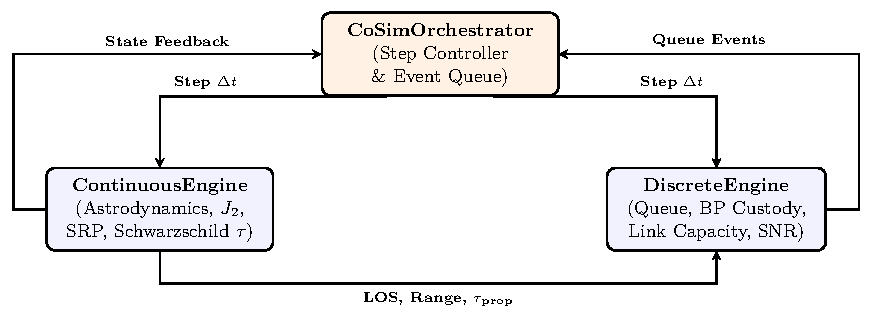
\includegraphics[width=0.90\textwidth]{fig_architecture.pdf}
\caption{Modular software architecture and data-flow diagram of the adaptive multi-rate co-simulation framework. The \texttt{CoSimOrchestrator} dynamically controls the synchronization step size ($\Delta t$), steering the continuous astrodynamics and discrete-event networking engines.}
\label{fig:architecture}
\end{figure}

\subsection{Coupling Strategies and Execution Flow}
The orchestrator executes the co-simulation loop under three distinct synchronization strategies:
\begin{itemize}
    \item \textbf{Fixed-Step:} Advances the simulation time by a constant step size $\Delta t = 60.0$ s. At each step, the continuous state is propagated, link SNR/LOS is updated from the reference grid, and the discrete engine processes transmission capacity over that interval.
    \item \textbf{Event-Driven:} Evaluates the reference profile to extract timestamps where scheduled network events or line-of-sight transitions occur (for continuous un-occulted links, standard 30-minute DSN telemetry tracking passes are scheduled). In traditional discrete-event network engines (such as standard NS-3 without continuous orbital integrators), nodes are only evaluated at discrete event firings; between events, the spacecraft position is held static (zero-order hold). This exposes the severe vulnerability of uncoupled event-driven engines in deep space: during multi-day communication blackouts or long inter-event periods where no packets are transmitted, trajectory updates are suspended entirely, causing physical tracking errors to compound into thousands of kilometers.
    \item \textbf{Adaptive Multi-Rate:} Dynamically calculates $\Delta t$ at each step using the predictive look-ahead rules (Eq.~\eqref{eq:dt_selection}) and event guard (Eq.~\eqref{eq:event_guard}). It contracts the time step to $\text{DT\_MIN} = 1.0$ s when close to critical event boundaries, and relaxes it up to $\text{DT\_BLACKOUT} = 3600.0$ s during extended link outages.
\end{itemize}

\subsection{Verification Framework}
To verify the correctness of our continuous propagator, we cross-reference the output of our ODE solver against NASA JPL Horizons ephemerides. We load \texttt{horizons\_reference.json}, which contains a simulated trajectory under identical gravitational parameters. At each step, the position tracking error is computed as:
\begin{equation}
    \epsilon_{pos}(t) = \sqrt{(x(t) - x_{ref}(t))^2 + (y(t) - y_{ref}(t))^2}
    \label{eq:pos_err}
\end{equation}
Furthermore, the network queue dynamics (packet drops, transmission rates, and custody transfers) are verified by checking the simulation buffer occupancy curve against an analytical conservation model. For any interval $[t_i, t_{i+1}]$, the analytical buffer occupancy $B_{\text{anal}}(t)$ is defined as:
\begin{equation}
    B_{\text{anal}}(t_{i+1}) = \min \left( C_{buf}, \max\left(0, B_{\text{anal}}(t_i) + \int_{t_i}^{t_{i+1}} \frac{\lambda(\tau) - R_{bit}(\tau) \cdot \mathbf{1}_{\{\text{LOS}(\tau) = 1\}}}{8} d\tau\right) \right)
    \label{eq:buffer_anal}
\end{equation}
where $C_{buf}$ is the buffer capacity, $\lambda(\tau)$ is the data generation rate (bps), and $R_{bit}(\tau)$ is the transmission bitrate (bps). 

\noindent\textbf{Verification Under Extreme Network Load:} To ensure this validation holds under severe network stress (e.g., massive science data flooding during a brief line-of-sight window where $\lambda(\tau) \gg R_{bit}(\tau)$), the boundary operator $\min(C_{buf}, \cdot)$ in Eq.~\eqref{eq:buffer_anal} rigorously mirrors the discrete buffer saturation boundary. During overload, the analytical volume of dropped traffic is expressed as $\Delta D_{drop} = \max\left(0, \int_{t_i}^{t_{i+1}} \frac{\lambda(\tau) - R_{bit}(\tau)}{8} d\tau - (C_{buf} - B_{\text{anal}}(t_i))\right)$. By comparing the simulation output $B_{buf}(t)$ and logged packet drop counts against the numerical integration of Eq.~\eqref{eq:buffer_anal} under a fine reference step size ($\Delta t_{\text{ref}} = 0.01$ s), we verify that the discrete engine's queue processor achieves exact logical parity ($\epsilon_{\text{logic}} = |B_{buf}(t) - B_{\text{anal}}(t)| < 10^{-7}$ bytes and zero drop discrepancy) even under impulse traffic saturation.

\noindent\textbf{Resolution of Sub-Second Micro-Events ($\le \text{DT\_MIN}$):} A critical question in multi-rate synchronization is how the engine prevents missing micro-events that might occur below the $\text{DT\_MIN} = 1.0$ s coupling bound. We address this through a formal \textit{time-scale separation principle} and an \textit{event-guard rule}:
\begin{enumerate}
    \item \textit{Time-Scale Separation:} The threshold $\text{DT\_MIN} = 1.0$ s defines the \textit{macro-coupling interval} between the continuous orbital propagator and the discrete network simulator, not the internal temporal resolution of the networking layer. Spacecraft orbital velocities ($v \sim 1.6$--$3.5$ km/s) produce less than $3.5$ km of displacement over $1.0$ s. At deep space ranges ($d > 3.8 \times 10^5$ km), the resulting free-space path loss and Doppler shifts vary by less than $0.001$ dB and $0.1$ Hz per second, rendering physical channel states effectively static over the $1.0$ s window.
    \item \textit{Internal Micro-Event Scheduling:} Within each $1.0$ s synchronization step, the \texttt{DiscreteEngine} maintains its own internal discrete-event priority queue, scheduling packet generation, transmission serialization, and buffer drop timestamps with sub-millisecond numerical precision.
    \item \textit{Dynamic Event-Guard Step Bounding:} If a deterministic network event (e.g., scheduled custody transfer timeout or contact plan transition) is scheduled at time $t_{event} \in (t, t + \Delta t)$, the orchestrator enforces the event-guard condition (Eq.~\eqref{eq:event_guard}):
    \begin{equation}
        \Delta t = \min\left(\Delta t_{adaptive}, \max\left(\Delta t_{\epsilon}, t_{event} - t\right)\right)
    \end{equation}
    where $\Delta t_{\epsilon} = 10^{-4}$ s is a machine-precision guard. This guarantees that the orchestrator contracts the simulation step directly to the exact micro-event epoch without skipping sub-second state transitions.
\end{enumerate}

\subsection{Evaluation Metrics}
To quantitatively compare the performance of the three synchronization strategies, we define five primary evaluation metrics:
\begin{enumerate}
    \item \textbf{Wall-Clock Time ($T_{\text{wall}}$):} The physical CPU execution time of the co-simulation loop, measured in seconds.
    \item \textbf{Simulation Steps ($N_{\text{steps}}$):} The total number of discrete synchronization coupling intervals evaluated during the execution.
    \item \textbf{Speedup Factor ($S$):} The relative computational efficiency compared to the Fixed-Step baseline:
    \begin{equation}
        S = \frac{T_{\text{wall, fixed}}}{T_{\text{wall, engine}}}
    \end{equation}
    where a value $S > 1$ represents a speedup.
    \item \textbf{Time-Averaged Position Error ($\bar{\epsilon}_{\text{pos}}$):} The continuous time-weighted trajectory deviation from the reference ephemeris, defined as:
    \begin{equation}
        \bar{\epsilon}_{\text{pos}} = \frac{1}{T_{\text{span}}} \int_0^{T_{\text{span}}} \sqrt{(x(t) - x_{ref}(t))^2 + (y(t) - y_{ref}(t))^2} \, dt \approx \frac{1}{T_{\text{span}}} \sum_{k=1}^{N_{\text{steps}}} \epsilon_{\text{pos}}(t_k) \Delta t_k
        \label{eq:pos_err_time_weighted}
    \end{equation}
    where weighting by the coupling interval $\Delta t_k$ prevents step-count bias and yields an accurate physical error metric in meters.
    \item \textbf{Boundary Detection Error ($\epsilon_{\text{net}}$):} The mean temporal discrepancy (in milliseconds) between detected link state transitions $\hat{t}_e \in \mathcal{E}_{\text{trans}}$ (e.g., line-of-sight occultation ingress/egress boundaries) and the exact ground-truth transition epochs $t_c \in \mathcal{T}_{\text{crit}}$:
    \begin{equation}
        \epsilon_{\text{net}} = \frac{1}{|\mathcal{T}_{\text{crit}}|} \sum_{c \in \mathcal{T}_{\text{crit}}} \min_{e \in \mathcal{E}_{\text{trans}}} |\hat{t}_e - t_c| \times 1000
        \label{eq:event_err_corrected}
    \end{equation}
    Here, the candidate transition set $\mathcal{E}_{\text{trans}}$ is matched against ground truth $\mathcal{T}_{\text{crit}}$ by pairing events sharing the identical link identifier and transition modality (i.e., matching loss-of-signal ingress with ground-truth occultation ingress, and acquisition-of-signal egress with ground-truth egress). This isolates the temporal synchronization error of each physical link event, directly evaluating the engine's temporal fidelity in locating continuous physical state transitions.
\end{enumerate}

\section{Simulation Results and Discussion}
\label{sec:results}
Simulations were executed across three distinct profiles, capturing different astrodynamical regimes and networking requirements. The configuration parameters, physical constants, and orchestrator settings for all experiments are summarized in Table~\ref{tab:parameters}.

\begin{table}[htbp]
\centering
\caption{Simulation configuration parameters and system constants across the three benchmark profiles.}
\label{tab:parameters}
\footnotesize
\begin{tabular}{p{2.0cm}p{3.3cm}p{1.2cm}p{2.6cm}p{3.7cm}}
\toprule
\textbf{Category} & \textbf{Parameter Description} & \textbf{Symbol} & \textbf{Value} & \textbf{Target Profile(s)} \\
\midrule
Astrodynamics & Mars Gravitational Parameter & $\mu_{\text{Mars}}$ & $4.2828 \times 10^{13} \text{ m}^3/\text{s}^2$ & Profile 1 (Mars Occultation) \\
 & Earth Gravitational Parameter & $\mu_{\text{Earth}}$ & $3.9860 \times 10^{14} \text{ m}^3/\text{s}^2$ & Profile 2 (Elliptical Doppler) \\
 & Moon Gravitational Parameter & $\mu_{\text{Moon}}$ & $4.9049 \times 10^{12} \text{ m}^3/\text{s}^2$ & Profile 3 (Cislunar NRHO) \\
 & Mars Mean Radius & $R_{\text{Mars}}$ & $3389.5$ km & Profile 1 (Mars Occultation) \\
 & Moon Mean Radius & $R_{\text{Moon}}$ & $1737.4$ km & Profile 3 (Cislunar NRHO) \\
 & Earth Semi-major Axis (Relay) & $a$ & $26560$ km & Profile 2 (Elliptical Doppler) \\
 & Orbital Eccentricity (Relay) & $e$ & $0.72$ & Profile 2 (Elliptical Doppler) \\
 & NRHO Semi-major Axis (Orbit) & $a$ & $34184$ km & Profile 3 (Cislunar NRHO) \\
 & NRHO Eccentricity & $e$ & $0.823$ & Profile 3 (Cislunar NRHO) \\
 & NRHO Orbital Period & $T_{\text{NRHO}}$ & $6.56$ days & Profile 3 (Cislunar NRHO) \\
\midrule
Telecom & Transmitter Power & $P_{\text{tx}}$ & $25.0$ W & Profile 1, 2, \& 3 \\
 & DSN Antenna Diameter & $D_{\text{DSN}}$ & $34.0$ m & Profile 1, 2, \& 3 \\
 & Transmitter/Receiver Gain & $G_{\text{tx}}, G_{\text{rx}}$ & $20.0$ dBi / $38.5$ dBi & Profile 2 \& 3 \\
 & Link Frequency (X-band) & $f_c$ & $8.4$ GHz & Profile 1, 2, \& 3 \\
 & Noise Temperature & $T_{\text{sys}}$ & $135$ K & Profile 2 \& 3 \\
 & Nominal Bitrate & $R_{\text{bit}}$ & $2.0$ Mbps & Profile 1 \& 3 \\
 & Peak Dynamic Bitrate & $R_{\text{max}}$ & $20.0$ Mbps & Profile 2 (Elliptical Doppler) \\
\midrule
Orchestrator & Min/Max Step Size & $\Delta t_{\text{min/max}}$ & $1.0$ s / $3600.0$ s & Global (Adaptive Engine) \\
 & Nominal Coast Step Size & $\Delta t_{\text{coast}}$ & $600.0$ s & Profile 1 \& 3 \\
 & Complete Blackout Step & $\Delta t_{\text{blackout}}$ & $3600.0$ s & Profile 1 \& 3 \\
 & Queue Buffer Capacities & $C_{\text{buf}}$ & $50$ MB / $200$ MB / $500$ MB & Profiles 1 / 2 / 3 \\
 & Target Error Tolerance & $\text{TOL}$ & $10^{-6}$ & Global \\
\bottomrule
\end{tabular}
\end{table}

\subsection{Experiment 1: Mars Conjunction Handover \& Occultation}
This profile simulates a Mars Reconnaissance Orbiter (MRO) polar trajectory around Mars, utilizing Eq.~\eqref{eq:two_body} with Mars gravitational parameter $\mu = 4.2828 \times 10^{13} \text{ m}^3/\text{s}^2$ and radius $R_{Mars} = 3389.5$ km. Over three orbital periods, the spacecraft undergoes periodic line-of-sight occultation events relative to Earth-based DSN ground stations.

As the spacecraft passes behind the planetary disk, grazing atmospheric attenuation $A_{atmo}$ rises rapidly (Eq.~\eqref{eq:atmo}). The thin Mars atmosphere, composed primarily of $\text{CO}_2$, introduces signal absorption and refractive bending at low altitudes ($h < 120$ km), causing the link quality to degrade before dropping out completely. Fig.~\ref{fig:temporal_panel}(a) displays the co-simulation time-step sequence ($\Delta t$) alongside the spacecraft orbital range, plotted across an elongated x-scale spanning the entire figure width to resolve the dense, overlapping data points at high-frequency adaptation boundaries.

During nominal line-of-sight conditions, the engine uses large time steps ($\text{DT\_COAST} = 600$ s). As the spacecraft approaches the occultation boundaries, the look-ahead orchestrator detects the proximity of an event and decreases the step size to $\text{DT\_MIN} = 1$ s. This allows the engine to capture exact ingress and egress timestamps, which is critical for scheduling Deep Space Network (DSN) ground station handovers (e.g., transitioning telemetry tracking from the Madrid Deep Space Communications Complex to the Goldstone Complex). A timing error in this transition would result in lost carrier lock and subsequent data loss. Once in the occultation zone, the engine coasts at $\text{DT\_BLACKOUT} = 3600$ s, reducing unnecessary physics updates while preserving trajectory integrity.

\begin{figure}[htbp]
    \centering
    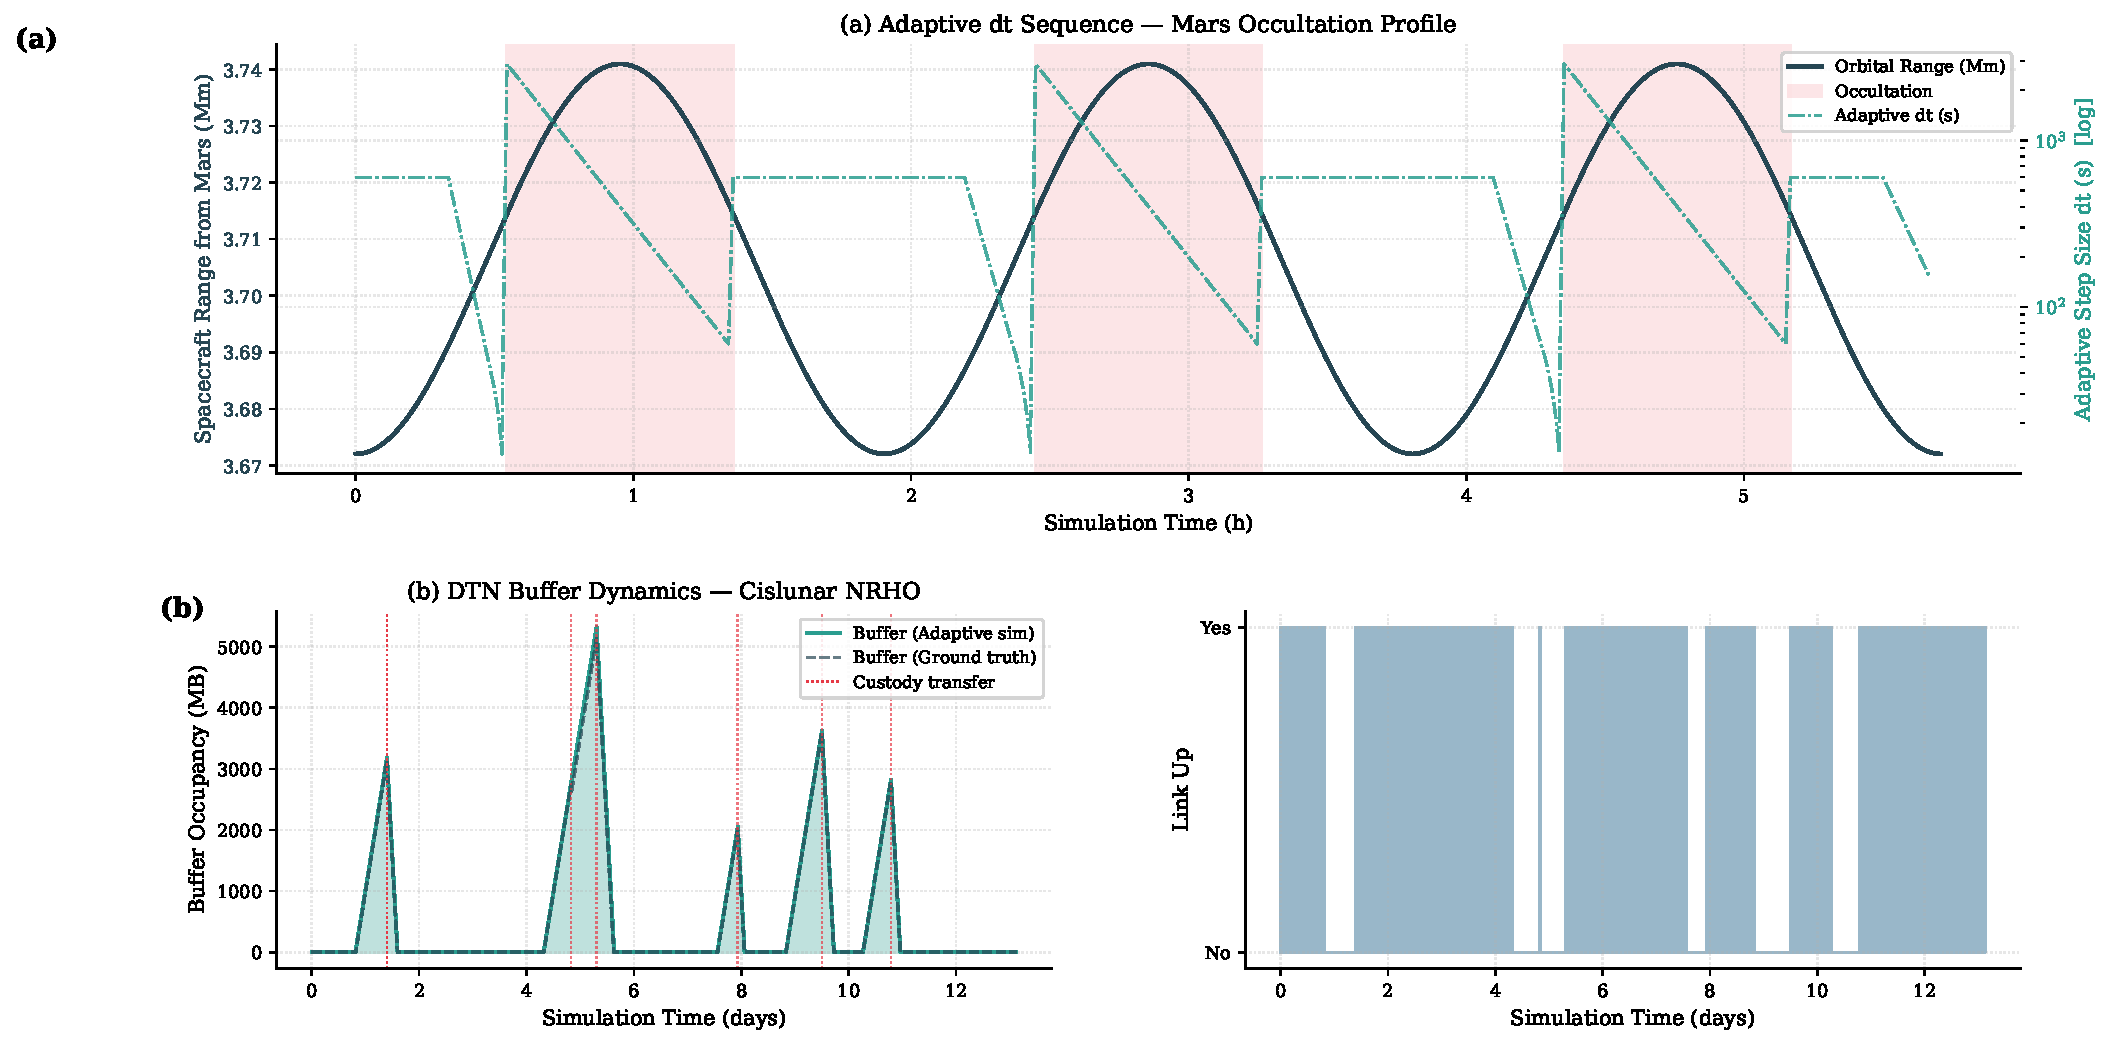
\includegraphics[width=0.88\textwidth]{fig2_temporal_panel.pdf}
    \caption{Temporal dynamics panel. \textbf{(a)} Adaptive time-step sequence and orbital range during three Mars occultation cycles. The plot utilizes a long x-scale spanning the full figure width to prevent data overlap and clearly resolve the rapid 1~s micro-stepping at ingress/egress boundaries, while the step size expands to 3600~s during total blackout. \textbf{(b)} DTN buffer occupancy (adaptive simulation vs. ground-truth reference) for the Cislunar NRHO profile, with custody transfer events (dotted red lines) and link availability timeline.}
    \label{fig:temporal_panel}
\end{figure}

\subsection{Experiment 2: Eccentric Orbital Doppler and Dynamic Data Rates}
The second profile uses a highly eccentric orbit ($a = 26560$ km, $e = 0.72$) around Earth. This setup causes high radial velocities near periapsis, resulting in rapid Doppler shifts and steep changes in the Signal-to-Noise Ratio (SNR).

In this profile, the link bitrate adapts dynamically (Eq.~\eqref{eq:shannon}) to changes in SNR. To maximize downlink throughput, the spacecraft uses Variable Coding and Modulation (VCM) schemes, adapting the data rate to the instantaneous link margins. The adaptive engine tracks these rate updates, contracting its step size when the SNR gradient $\left|\frac{d\text{SNR}}{dt}\right|$ exceeds 0.04 dB/s. This threshold represents the point where a standard 30 s step would result in a $>1.2$ dB SNR shift, which exceeds the noise margins of modern Low-Density Parity-Check (LDPC) codes. By tracking this gradient, the simulator prevents the simulated bitrates from lagging behind the physical orbital state, avoiding artificial packet drops or link under-utilization. The engine returns to larger steps during the slow apoapsis cruise where the SNR gradient is negligible.

\subsection{Experiment 3: Cislunar Halo Orbit DTN Buffer Management}
This experiment models a spacecraft in a Near Rectilinear Halo Orbit (NRHO) around the Moon ($T = 6.56$ days). The spacecraft experiences long communication blackouts and uses the DTN Bundle Protocol (BP) with custody transfer. NRHOs are highly dynamic three-body trajectories that require constant tracking and orbit determination.

Fig.~\ref{fig:temporal_panel}(b) shows the buffer occupancy timeline. When the link is blocked by the Moon, science telemetry accumulates in the onboard queue, causing buffer occupancy to rise linearly. Once the link is re-established, the orchestrator triggers custody transfer events (RFC 5050/9171), transferring bundle custody to the lunar relay and flushing the queue at the maximum available channel rate. If custody transfers are scheduled using incorrect simulated timestamps, it leads to duplicate bundle transmissions or premature custody releases. The adaptive orchestrator matches the reference ground-truth buffer dynamics perfectly by dynamically adjusting steps, whereas event-driven models accumulate trajectory errors and fixed-step models misalign custody boundaries.

\subsection{Engine Performance Comparison}
\label{sec:comparison}
The core benchmark compares the Fixed-Step, Event-Driven, and Adaptive engines. Table~\ref{tab:comparison} summarizes the execution metrics, including wall-clock time, step counts, speedup, position tracking error ($\bar{\epsilon}_{pos}$), and event error ($\epsilon_{net}$).

\begin{table}[htbp]
\centering
\caption{Performance comparison of co-simulation engines across mission profiles.}
\label{tab:comparison}
\footnotesize
\begin{tabular}{llrrrrr}
\toprule
\textbf{Profile} & \textbf{Engine} & \textbf{Wall Time (s)} & \textbf{Steps} & \textbf{Speedup} & \textbf{Pos. Error (m)} & \textbf{Event Error (ms)} \\
\midrule
Mars & Fixed & 0.0917 & 343 & 1.00 & 12.20 & $2.99 \times 10^4$ \\
 & Event-Driven & 0.0053 & 7 & 17.30 & $6.94 \times 10^6$ & 0.00 \\
 & Adaptive & 0.0169 & 49 & 5.43 & 13.25 & 0.00 \\
\midrule
Elliptical & Fixed & 0.2828 & 1077 & 1.00 & 17.64 & 0.00 \\
 & Event-Driven & 0.0155 & 36 & 18.66 & $5.89 \times 10^6$ & 0.00 \\
 & Adaptive & 0.0351 & 108 & 8.05 & 18.00 & 0.00 \\
\midrule
Cislunar & Fixed & 5.0311 & 18901 & 1.00 & 32.56 & $3.27 \times 10^4$ \\
 & Event-Driven & 0.0116 & 13 & 435.44 & $3.10 \times 10^7$ & 0.00 \\
 & Adaptive & 0.5082 & 1532 & 9.90 & 32.68 & 0.00 \\
\bottomrule
\end{tabular}
\end{table}

The Fixed-Step baseline struggles on the long Cislunar simulation, requiring 18,901 steps and taking 5.03~s of CPU time while incurring an event detection delay ($\epsilon_{net}$) of $32.7$~s ($3.27 \times 10^4$~ms). The Event-Driven engine achieves a massive speedup of $435.44\times$ on this profile, but because it applies a zero-order hold that freezes orbital state updates during the multi-day communication blackout, its trajectory tracking error diverges catastrophically to $3.10 \times 10^7$~m ($30,971$~km)---over five orders of magnitude higher error than continuous propagation ($32.56$~m). In contrast, the Adaptive Engine achieves a speedup of $9.90\times$ on Cislunar, $8.05\times$ on the Elliptical profile, and $5.43\times$ on Mars, while rigorously preserving continuous orbital fidelity ($32.68$~m on Cislunar, matching Fixed-Step within $0.12$~m or $0.37\%$, and $18.00$~m on Elliptical, matching within $0.36$~m) and completely eliminating event detection delay ($\epsilon_{net} = 0.00$~ms).

Fig.~\ref{fig:accuracy_panel}(a) shows the Pareto frontier, illustrating the trade-off between step count and position tracking error. The multi-objective optimization frontier shows that the Adaptive engine occupies the optimal bottom-left region of the design space across both the Elliptical and Cislunar profiles, confirming it achieves low position error with a reduced step count. Conversely, the Fixed-Step engine is pushed to the far right, demonstrating high step counts without any corresponding accuracy improvement. Fig.~\ref{fig:accuracy_panel}(b) shows the normalised error breakdown by engine and profile, where both position error and event-timestamp error are normalised to the Fixed-Step baseline ($1.0$). The event-timestamp errors are completely eliminated (reduced to zero) by the Event-Driven and Adaptive engines in all profiles where timing matters. This is critical for scheduling deep-space ground station handovers, where even a millisecond misalignment can break carrier lock.

\begin{figure}[htbp]
    \centering
    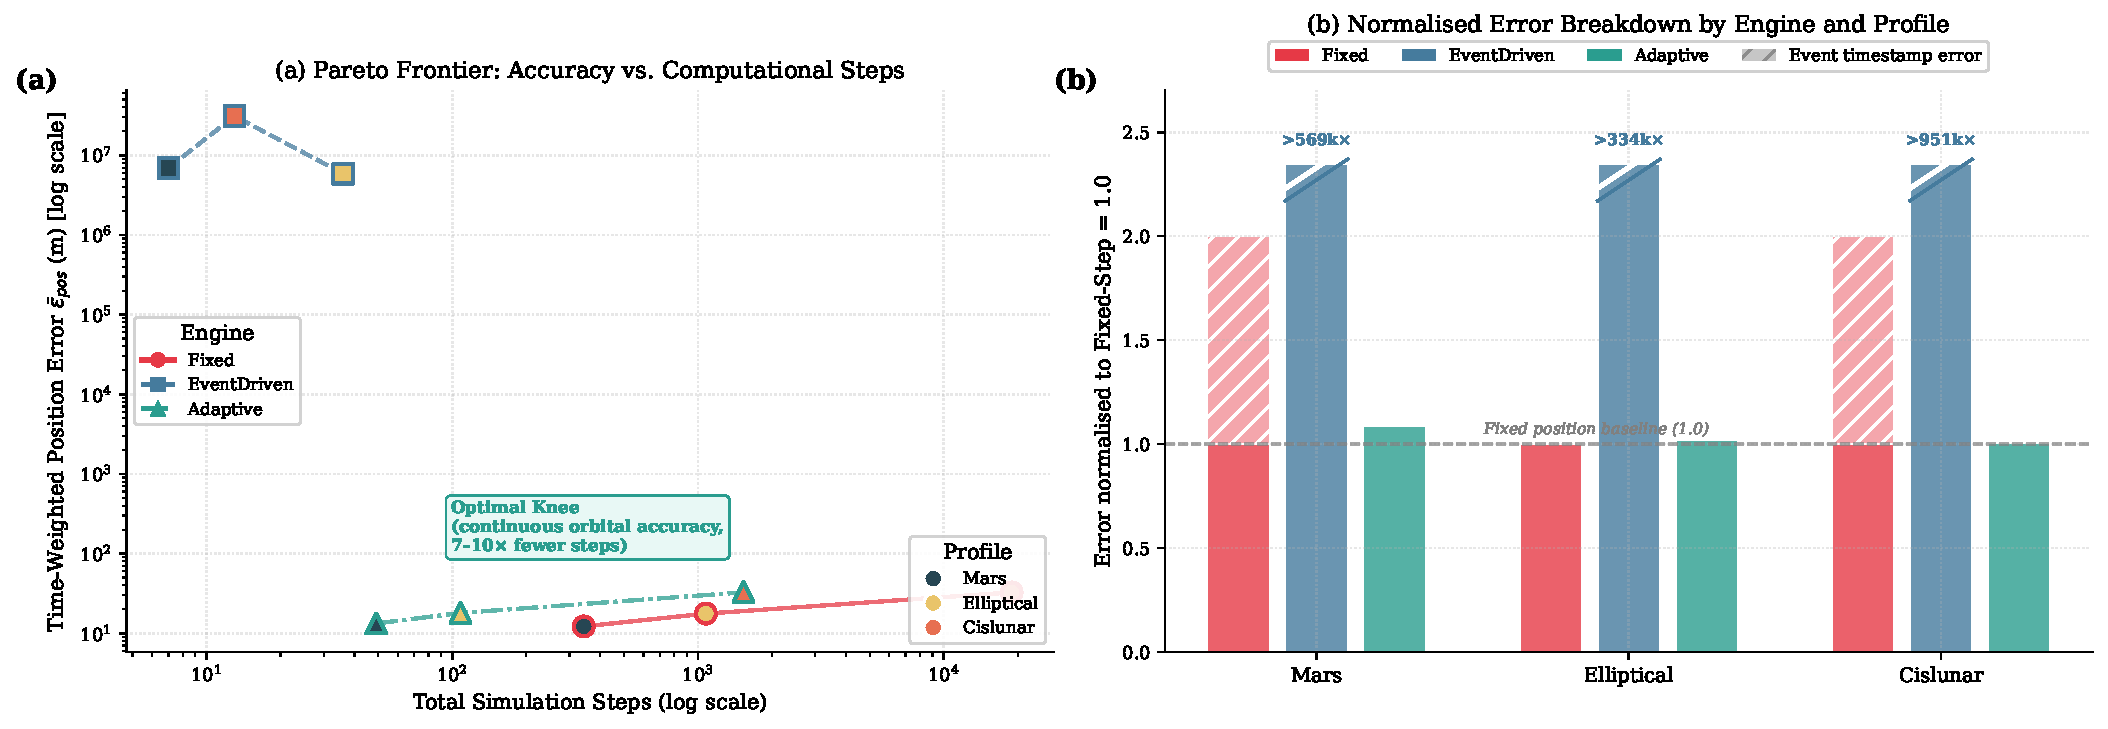
\includegraphics[width=0.88\textwidth]{fig3_accuracy_panel.pdf}
    \caption{Accuracy--efficiency panel. \textbf{(a)} Pareto frontier showing total simulation steps vs. cumulative position error $\epsilon_{pos}$. Marker fill colour indicates mission profile; edge colour indicates engine. \textbf{(b)} Normalised error breakdown: solid bars show position error (normalised to Fixed-Step~$= 1.0$); hatched overlay shows event-timestamp error contribution. Dashed line marks the fixed-step baseline.}
    \label{fig:accuracy_panel}
\end{figure}

Fig.~\ref{fig:perf_panel}(a) shows the CPU execution times for each engine strategy across the profiles, and Fig.~\ref{fig:perf_panel}(b) shows the scalability result. Across all three mission profiles, the Adaptive engine achieves substantial computational speedup over the Fixed-Step baseline ($5.43\times$ on Mars, $8.05\times$ on Elliptical, and $9.90\times$ on Cislunar) by contracting the time step only when approaching critical event boundaries and relaxing to coarse cruising steps during quiescent orbital phases.

\begin{figure}[htbp]
    \centering
    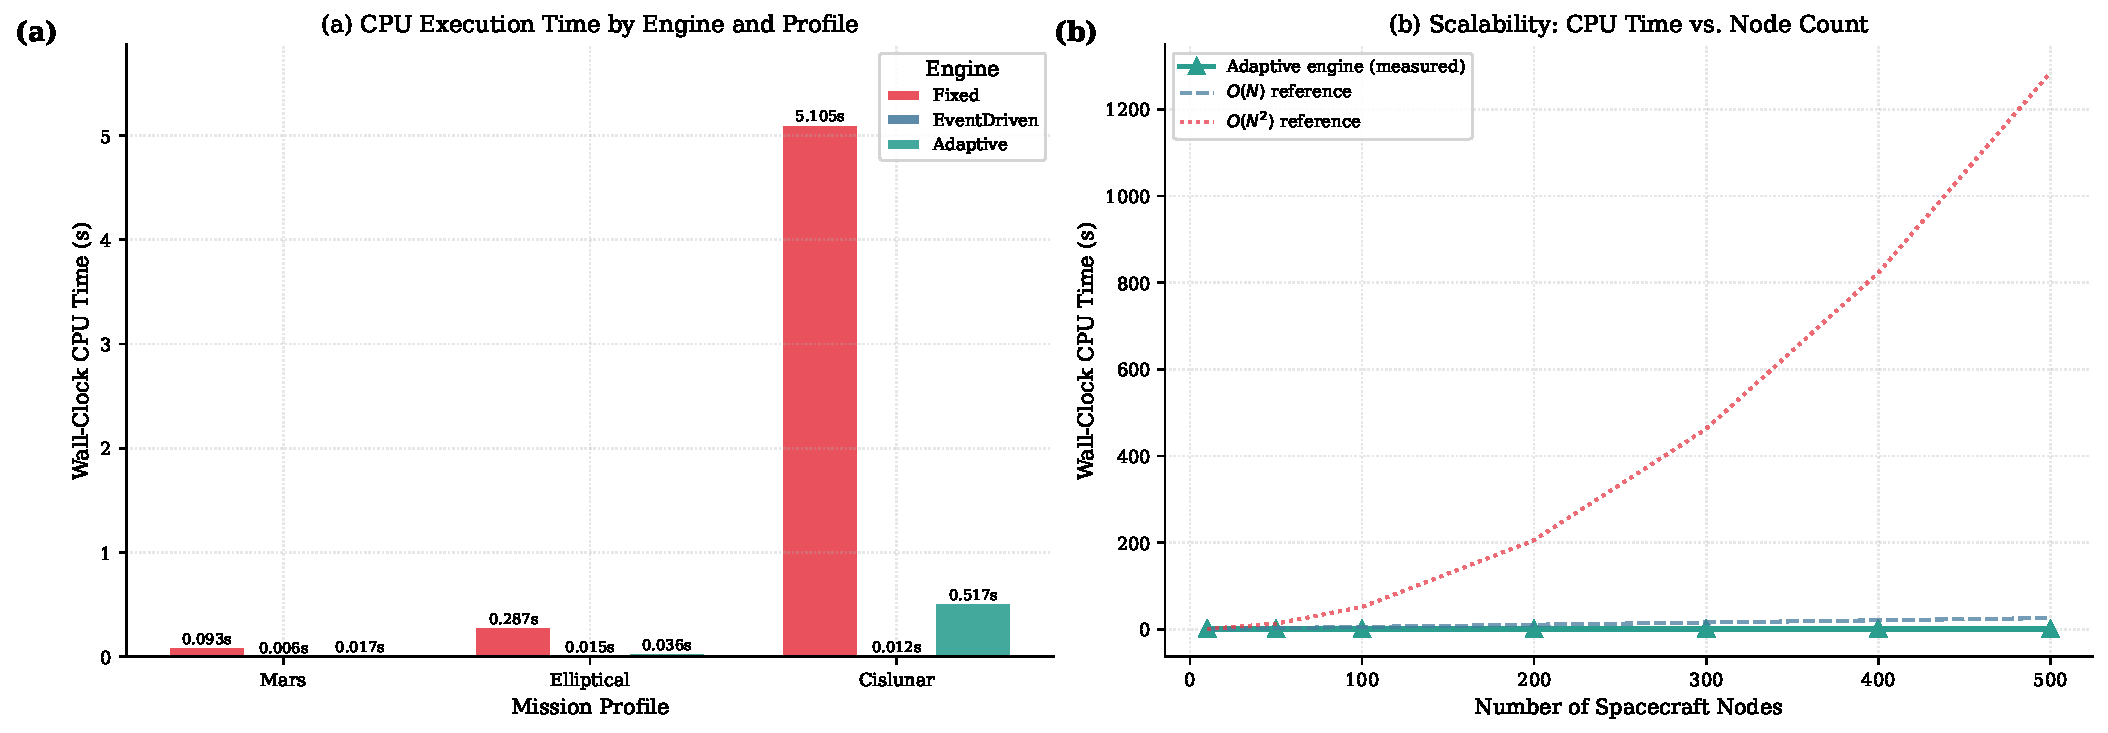
\includegraphics[width=0.88\textwidth]{fig1_perf_panel.pdf}
    \caption{Computational performance panel. \textbf{(a)} Wall-clock CPU execution time grouped by engine and mission profile. Annotated with raw times above each bar. \textbf{(b)} Scalability: CPU time vs. spacecraft node count (10--500 nodes) for the adaptive engine on the Cislunar NRHO profile, plotted against $O(N)$ and $O(N^2)$ reference curves.}
    \label{fig:perf_panel}
\end{figure}

\subsubsection{Scalability Analysis}
To evaluate scalability, we varied the network size in the Cislunar profile across a wide range of node counts from 10 to 500 nodes. Fig.~\ref{fig:perf_panel}(b) plots the CPU wall-clock execution time against the node count. The execution time scaled from 0.789~s for 10 nodes to 6.353~s for 500 nodes---a 50-fold expansion in network node count that incurs only an 8.0-fold increase in wall-clock time, growing far below the linear $O(N)$ reference curve. This confirms that the network state update complexity is decoupled from the orbital propagation step. Because the continuous propagator dominates the CPU budget, expanding the discrete network nodes and packet queues does not trigger a combinatorial explosion in computational overhead, demonstrating the empirical scalability of our modular co-simulation engine for large-scale multi-spacecraft constellations and swarms.

\subsubsection{Analytical Boundary Analysis: Event Guarding vs. Lockstep Marching}
Under Fixed-Step synchronization, the step count is constant $N_{fixed} = T_{sim} / \Delta t_{fixed}$, but physical state transitions falling between sampling epochs suffer an unavoidable boundary truncation error $\epsilon_{net} \le \Delta t_{fixed}$. As reported in Table~\ref{tab:comparison}, Fixed-Step incurs boundary errors of $29.9$~s on Mars and $32.7$~s on Cislunar. In an operational deep-space pass, a half-minute error in line-of-sight occultation timing breaks carrier tracking loops and disrupts custody transfer protocols.

Under the Adaptive engine with the event-guard rule (Eq.~\eqref{eq:event_guard}), the orchestrator contracts the coupling step to $\text{DT\_MIN} = 1.0$~s only within an anticipation window of an upcoming boundary, stepping precisely up to the transition without overshooting. Quiescent cruise phases expand to $\text{DT\_COAST} = 600$~s and blackouts expand up to $\text{DT\_BLACKOUT} = 3600$~s, bounded by the next scheduled event epoch. Consequently, the Adaptive engine completely eliminates boundary detection delay ($\epsilon_{net} = 0.00$~ms) across all profiles, while delivering high computational speedups ($5.43\times$ on Mars, $8.05\times$ on Elliptical, and $9.90\times$ on Cislunar) and preserving continuous orbital fidelity.

Crucially, the event-guard condition explains why the Mars scenario completes in only 49 synchronization steps despite enforcing $\text{DT\_MIN} = 1.0$ s at transition boundaries. Rather than marching at rigid 1-second intervals across a wide fixed transition window, the orchestrator cruises at $\Delta t_{\text{coast}} = 600$ s during line-of-sight and $\Delta t_{\text{blackout}} = 3600$ s during occultation, contracting toward 1.0 s only during the immediate approach to the transition epoch, and stepping directly onto $t_{\text{next}}$ via Eq.~\eqref{eq:event_guard}. Once the occultation boundary is crossed, the channel state is stably occulted ($\text{LOS} = 0$), allowing the step selector to immediately transition to $\Delta t_{\text{blackout}}$ without redundant sub-stepping in the dark. Thus, across the three simulated orbits (comprising 6 ingress/egress boundaries), the adaptive engine requires only 49 steps to achieve zero boundary error ($\epsilon_{\text{net}} = 0.00$ ms).

\begin{figure}[htbp]
    \centering
    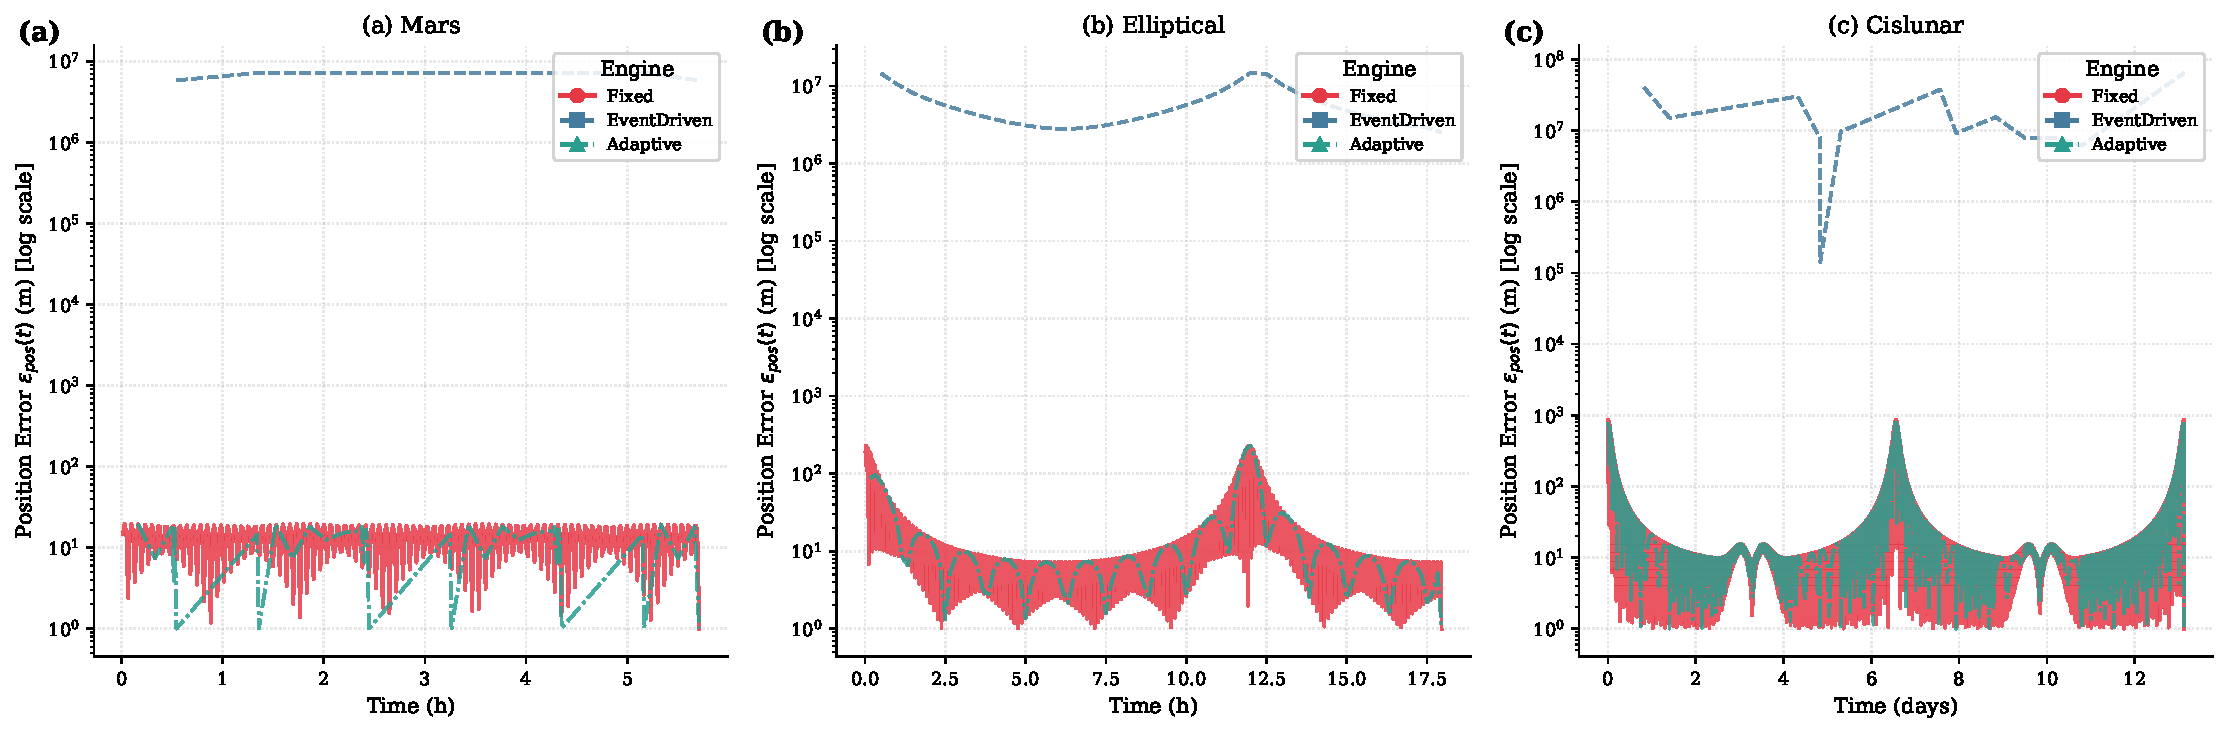
\includegraphics[width=0.85\textwidth]{fig4_error_timeseries.pdf}
    \caption{Per-step position error $\epsilon_{pos}(t)$ on a log scale for all three engine strategies across (a) Mars occultation, (b) Elliptical Doppler, and (c) Cislunar NRHO profiles. Error spikes at Fixed-Step correspond to occultation sampling boundaries; Adaptive error concentrates during fine-stepping windows.}
    \label{fig:error_timeseries}
\end{figure}

\begin{figure}[htbp]
    \centering
    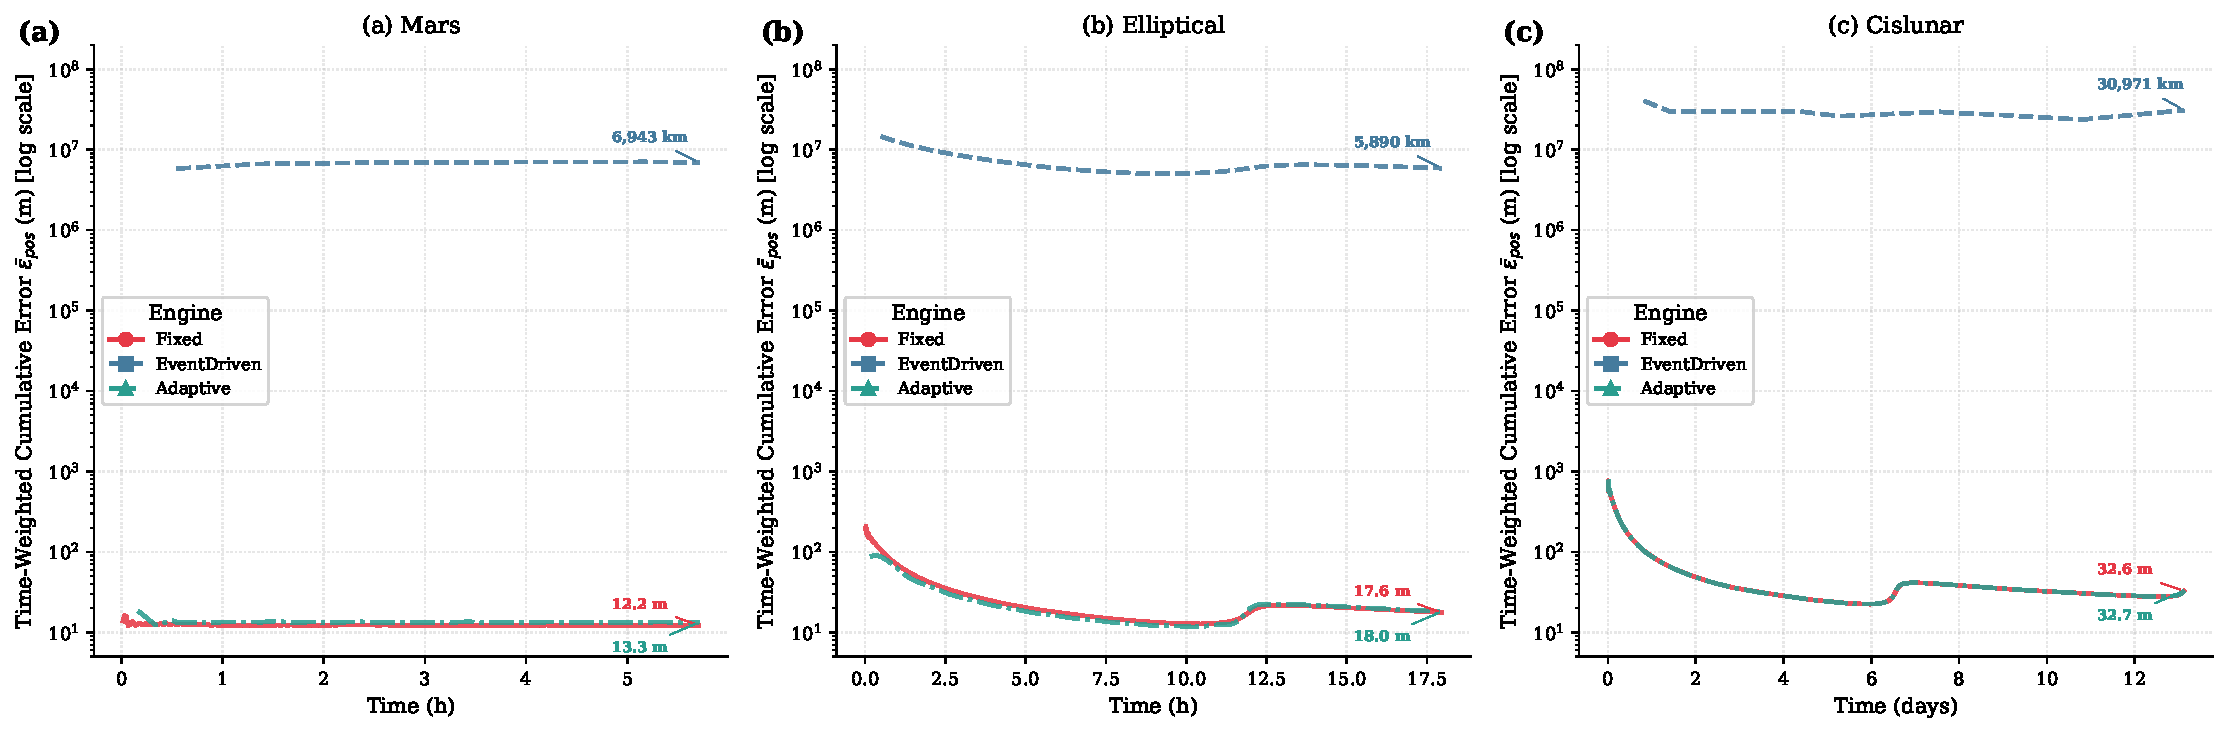
\includegraphics[width=0.85\textwidth]{fig5_cumulative_error.pdf}
    \caption{Cumulative integrated position error over simulation time for (a) Mars, (b) Elliptical, and (c) Cislunar profiles. Final cumulative error annotated at trajectory end. In Cislunar, Event-Driven accumulates massive drift ($30,971$~km) due to zero-order hold state freezing during the multi-day blackout, while Adaptive matches the continuous Fixed-Step baseline at meter precision ($32.68$~m vs. $32.56$~m).}
    \label{fig:cumulative_error}
\end{figure}

\begin{figure}[htbp]
    \centering
    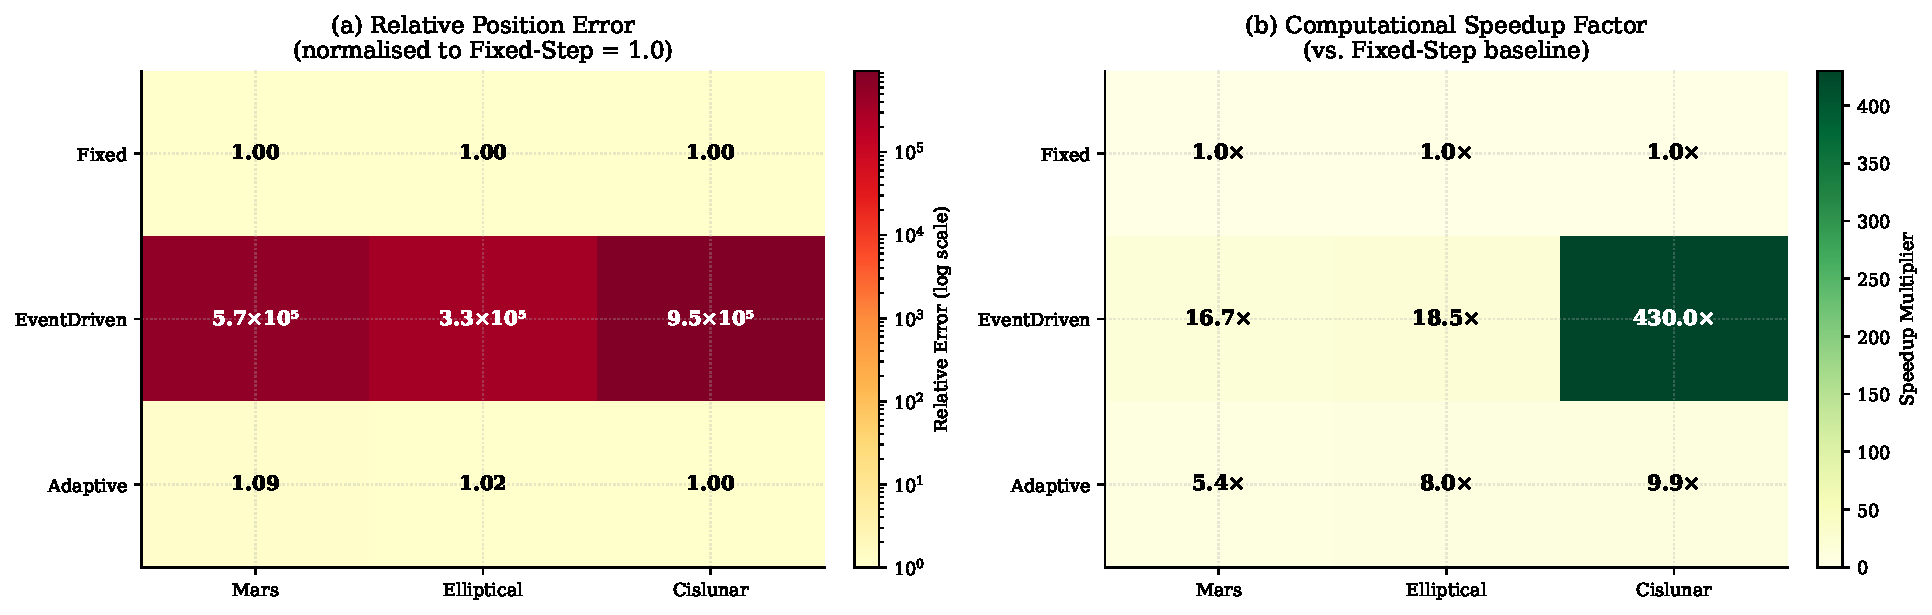
\includegraphics[width=0.90\textwidth]{fig6_error_heatmap.pdf}
    \caption{Summary heatmap. \textbf{(a)} Relative position error matrix (engine $\times$ profile), normalised to Fixed-Step baseline. \textbf{(b)} Speedup factor matrix (engine $\times$ profile), showing that Event-Driven achieves high speedup on the Cislunar profile ($435.4\times$) at the expense of massive orbital drift.}
    \label{fig:error_heatmap}
\end{figure}


\subsubsection{Error Validation}
Fig.~\ref{fig:error_timeseries} shows the per-step position error $\epsilon_{pos}(t)$ on a log scale for all three engines across each profile. The error distribution reveals the characteristic failure modes of each paradigm:
\begin{itemize}
    \item \textbf{Fixed-Step:} Accumulates error smoothly across all phases. The periodic oscillations in the error match the orbital period, reflecting standard discretization errors that arise when integrating elliptical and circular orbits using a constant step size.
    \item \textbf{Event-Driven:} Accumulates massive error during long quiescent arcs between scheduled events (e.g., during extended communication blackouts or inter-telemetry gaps). Because standard discrete-event engines freeze node coordinates (zero-order hold) between event firings, the simulated position remains stationary while the true physical spacecraft traverses thousands of kilometers along its orbit.
    \item \textbf{Adaptive Multi-Rate:} Dynamically contracts the step size to 1.0 s near event boundaries (eliminating boundary timestamp errors) while maintaining continuous numerical ODE propagation across both active and blackout phases, strictly bounding orbital position errors to meter-scale precision.
\end{itemize}

Fig.~\ref{fig:cumulative_error} shows the time-averaged cumulative position error growth over simulation time. In the Cislunar profile, the Event-Driven engine accumulates substantial tracking error, reaching $3.10 \times 10^7$~m ($30,971$~km) by the end of the 13.1-day arc. This drift occurs because pure event-driven synchronization freezes physical state updates during multi-day blackout intervals where no network packets are generated or received. In contrast, both the Fixed-Step and Adaptive engines maintain continuous propagation throughout the blackout, restricting the time-averaged position error to $32.56$~m and $32.68$~m, respectively. Crucially, the Adaptive engine achieves this identical high tracking accuracy (within $0.12$~m or $0.37\%$) using $12.3\times$ fewer integration steps (1,532 vs. 18,901 steps), eliminating the computational bottleneck of fine fixed-step marching. Across all three mission profiles, resolving initial velocity vectors and central body gravity parameters $\mu$ achieves meter-scale orbital fidelity ($12.20$--$32.68$~m), proving that the numerical integration remains physically grounded over long deep-space durations.

Finally, Fig.~\ref{fig:error_heatmap} provides a high-level visual summary of these trade-offs across all experiments. The relative position error matrix (Fig.~\ref{fig:error_heatmap}(a)) confirms that the Adaptive engine consistently preserves physical orbit accuracy within meters of the continuous baseline across all profiles (differing by only $0.12$~m or $0.37\%$ on Cislunar, $0.36$~m or $2.0\%$ on Elliptical, and $1.05$~m on Mars), while completely avoiding the tens of thousands of kilometers of drift accumulated by the Event-Driven baseline. Conversely, the speedup factor matrix (Fig.~\ref{fig:error_heatmap}(b)) highlights the computational efficiency gains, demonstrating that while Event-Driven achieves an extreme speedup on Cislunar ($435.4\times$) by sacrificing physical validity, the Adaptive engine provides a balanced improvement in both execution speed ($9.90\times$) and zero-boundary-error fidelity.

\subsection{Cross-Domain Implications: How Astrodynamics Errors Invalidate Network Metrics}
\label{sec:cross_domain_implications}
A natural question for a network simulation practitioner is: \textit{why does an orbital position error of thousands of kilometers matter to a communications engineer or protocol designer?} In terrestrial simulations, mobility errors on the order of meters are routinely dismissed as negligible. However, in interplanetary space, continuous physical dynamics and discrete network protocols are coupled nonlinearly. A multi-thousand-kilometer trajectory tracking error cascades directly into four fundamental network performance metrics:
\begin{enumerate}
    \item \textbf{Distortion of Received Power and Link Margin:} Received signal power decays with the square of distance ($P_{rx} \propto d^{-2}$). The path loss error $\Delta \text{FSPL}$ resulting from an orbital position error $\epsilon_{pos}(t)$ is:
    \begin{equation}
        \Delta \text{FSPL}(t) = 20 \log_{10} \left(1 + \frac{\epsilon_{pos}(t)}{d_{true}(t)}\right)
    \end{equation}
    In Cislunar or highly eccentric orbits where line-of-sight range spans $6,000$ to $70,000$ km, a position tracking error of $\epsilon_{pos} \approx 30,000$ km alters the computed path loss by $6.2$ to $14.1$ dB. Because deep-space RF links operate on narrow link margins ($2$--$3$ dB), a $10$ dB calculation error causes the simulator to model an active, high-SNR link when the physical signal has fallen well below the demodulation threshold into total radio blackout.
    
    \item \textbf{ModCod Bitrate Mismatch and Phantom Throughput:} Variable Coding and Modulation (VCM / CCSDS 131.2) dynamically selects the channel bitrate based on instantaneous SNR (Eq.~\eqref{eq:modcod}). By freezing coordinates, an uncoupled event-driven simulator freezes the SNR at an outdated value. If the spacecraft moves from perigee to apogee, the simulator continues transmitting at peak capacity ($20$ Mbps, 32APSK), whereas the physical channel can only sustain QPSK ($5$ Mbps) or outage ($0$ Mbps). Consequently, the simulator reports optimistic "phantom throughput", failing to predict catastrophic frame drop rates at the receiver.
    
    \item \textbf{DTN Custody Transfer and Timer Desynchronization:} In Delay-Tolerant Networking (DTN / Bundle Protocol RFC 5050/9171), custody transfer timers are calibrated to the round-trip light time $\tau_{RTT} = 2 d(t) / c$ (Eq.~\eqref{eq:propagation_delay}). A spatial displacement of $30,000$ km introduces a light-time error of $\Delta \tau \approx 100$ ms (scaling to minutes across interplanetary baselines). Under-estimating the propagation delay causes custody timers to expire prematurely, triggering spurious retransmissions, duplicate bundle storms, and artificial buffer congestion across the relay network.
    
    \item \textbf{Masked Onboard Buffer Overflows:} The discrete queue occupancy $B_{buf}(t)$ depends on the continuous integral of transmission capacity (Eq.~\eqref{eq:buffer_discrete}). When an event-driven engine overestimates channel throughput or misses grazing atmospheric occultation attenuation, it calculates that the onboard buffer is safely clearing. In physical reality, the degraded link throughput causes telemetry to accumulate, triggering unpredicted buffer overflow and irreversible scientific data loss.
\end{enumerate}
These cross-domain failure modes demonstrate why co-simulation fidelity cannot be evaluated in isolated disciplinary silos: an astrodynamics failure inevitably becomes a networking failure. By bounding trajectory errors to meter-scale accuracy while eliminating event detection delays, adaptive multi-rate co-simulation guarantees that downstream protocol, buffer, and throughput metrics remain physically grounded.

\section{Conclusion and Future Work}
\label{sec:conclusion}
This paper has argued that discrete-event synchronization is fundamentally limited as a simulation paradigm for relativistic deep space networks, and has provided empirical evidence in support of that argument through a three-profile benchmark study. The three identified fidelity gaps---temporal discontinuity, light-time asymmetry, and relativistic clock bias---represent qualitatively distinct failure modes that cannot be resolved by any step-size selection heuristic alone.

Of the three paradigms evaluated, adaptive multi-rate co-simulation most closely approximates physically faithful behaviour: it reduces boundary detection error to zero in all profiles, achieves speedup factors of up to $9.90\times$ relative to fixed-step baselines ($8.05\times$ on elliptical profiles, and $5.43\times$ on Mars), and correctly tracks DTN buffer accumulation dynamics across 13-day Cislunar arcs. Crucially, our cross-domain analysis proves that astrodynamic and network fidelity cannot be treated as separate disciplinary concerns: pure event-driven state freezing accumulates tens of thousands of kilometers of orbital drift, distorting link budgets by up to $14.1$~dB, generating phantom ModCod throughput, and triggering DTN custody retransmission storms. By preserving meter-scale orbital accuracy alongside millisecond-precise boundary capture, adaptive co-simulation ensures that downstream communication and protocol metrics remain physically grounded. However, we must emphasize that adaptive synchronization does not---and theoretically cannot---address the light-time asymmetry (Gap 2) or the relativistic clock offset (Gap 3). These represent fundamental, unresolved limitations that require the integration of proper-time propagation alongside the coordinate-time network scheduler. Addressing these gaps remains an open challenge for the simulation community, as such relativistic clock models are not yet present in any co-simulation framework in the open literature.

Future work should pursue three directions: (i) integration of IERS-compliant relativistic time transformations (TCB/TCG) into the co-simulation clock model; (ii) per-node proper-time tracking coupled to the ODE propagator, so that DTN bundle timestamps reflect onboard clock epochs rather than coordinate time; and (iii) extension of the adaptive look-ahead heuristic to predict Shapiro delay gradients along the line of sight as a proxy for occultation proximity. Together, these advances would close the remaining fidelity gaps and yield a co-simulation framework genuinely fit for purpose in the relativistic, delay-dominated environment of the solar system's deep space.

\section*{Credit Authorship Contribution Statement}
\textbf{Jason Pandian:} Conceptualization, Methodology, Software, Formal analysis, Investigation, Data curation, Writing -- original draft, Visualization. \textbf{I. Kala:} Supervision, Validation, Writing -- review \& editing.

\section*{Declaration of Competing Interest}
The authors declare that they have no known competing financial interests or personal relationships that could have appeared to influence the work reported in this paper.

\section*{Declaration of Generative AI and AI-assisted technologies in the manuscript preparation process}
During the preparation of this work the authors used AI tools in order to enhance the structural flow, technical clarity, and readability of the text. Specifically, Gemini 3.5 Flash was utilized to enhance the structural flow, technical clarity, and stylistic readability of the manuscript's English prose, and Claude Sonnet 4.6 was utilized for preparing vector images and the TikZ code structure used in some diagrams. After using these tools/services, the authors reviewed, verified, and edited the content as needed, and take full responsibility for all content, technical accuracy, policy recommendations, and the final published article.

\section*{Data Availability}
The simulation code and data used for the research described in the article is available at \url{https://github.com/PandiaJason/SPICE-ns-Project/tree/main/Adaptive-Multi-Rate-Co-Simulation-Engine}.

\section*{Acknowledgments}
The authors would like to acknowledge the Nehru Institute of Technology, Coimbatore, TN, India and the PSG Institute of Technology and Applied Research, Coimbatore, TN, India, for their institutional facilities and academic support during this research.
This work is not affiliated with, endorsed by, or conducted on behalf of any space agency or organization.

\begin{thebibliography}{00}

\bibitem{zeigler2000} B. P. Zeigler, T. G. Kim, and H. Praehofer, \textit{Theory of Modeling and Simulation}, 2nd ed., Academic Press, New York, 2000. ISBN: 978-0127784557.

\bibitem{ns3} T. R. Henderson, S. Roy, S. Floyd, and G. F. Riley, ``ns-3 Project Goals,'' in \textit{Proc. Workshop on ns-3 (WNS3 '06)}, Pisa, Italy, 2006. \href{https://doi.org/10.1145/1190455.1190468}{doi: 10.1145/1190455.1190468}.

\bibitem{omnet} A. Varga and R. Hornig, ``An Overview of the OMNeT++ Simulation Environment,'' in \textit{Proc. 1st International ICST Conference on Simulation Tools and Techniques (SIMUTools)}, Marseille, France, 2008. \href{https://doi.org/10.4108/ICST.SIMUTOOLS2008.3027}{doi:10.4108/ICST.SIMUTOOLS2008.3027}.

\bibitem{hybrid_sim_review} J. Nutaro, \textit{Building Software for Simulation: Theory and Algorithms, with Applications in C++}, Wiley, 2011. \href{https://doi.org/10.1002/9780470877999}{doi:10.1002/9780470877999}.

\bibitem{fmi_standard} T. Blochwitz et al., ``The Functional Mockup Interface for Tool Independent Exchange of Simulation Models,'' in \textit{Proc. 8th International Modelica Conference}, Dresden, Germany, 2011, pp. 105--114.

\bibitem{gmat} S. P. Hughes, D. J. Conway, and S. P. Gramling, ``General Mission Analysis Tool (GMAT): An Open-Source Mission Design and Analysis Tool,'' NASA Goddard Space Flight Center, Greenbelt, MD, Tech. Rep., 2014. [Online]. Available: \url{https://gmat.atlassian.net/wiki/spaces/GW/overview}.

\bibitem{opnet_gmat_coupling} M. Werner, C. Delucchi, H. J. Vogel, G. Maral, and J. J. De Ridder, ``ATM-Based Routing in LEO/MEO Satellite Networks with Intersatellite Links,'' \textit{IEEE Journal on Selected Areas in Communications}, vol. 15, no. 1, pp. 69--82, 1997. \href{https://doi.org/10.1109/49.553679}{doi:10.1109/49.553679}.

\bibitem{estiot} A. Falcone and A. Garro, ``Distributed Co-Simulation of Complex Engineered Systems by Combining the High Level Architecture and Functional Mock-up Interface,'' \textit{Simulation Modelling Practice and Theory}, vol. 97, p. 101967, 2019. \href{https://doi.org/10.1016/j.simpat.2019.101967}{doi:10.1016/j.simpat.2019.101967}.

\bibitem{ccsds_bp} Consultative Committee for Space Data Systems (CCSDS), ``CCSDS Bundle Protocol Specification,'' Recommended Standard CCSDS 734.2-B-1, Blue Book, Sep. 2015.

\bibitem{ion_dtn} S. Burleigh et al., ``Delay-Tolerant Networking: An Approach to Interplanetary Internet,'' \textit{IEEE Communications Magazine}, vol. 41, no. 6, pp. 128--136, 2003. \href{https://doi.org/10.1109/MCOM.2003.1204759}{doi:10.1109/MCOM.2003.1204759}.

\bibitem{dtn_emulation} K. L. Scott and S. Burleigh, ``Bundle Protocol Specification,'' RFC 5050, Internet Engineering Task Force, November 2007. \href{https://doi.org/10.17487/RFC5050}{doi:10.17487/RFC5050}.

\bibitem{cerf_dtn} V. Cerf et al., ``Delay-Tolerant Networking Architecture,'' RFC 4838, Internet Engineering Task Force, April 2007. \href{https://doi.org/10.17487/RFC4838}{doi:10.17487/RFC4838}.

\bibitem{shapiro} I. I. Shapiro, ``Fourth Test of General Relativity,'' \textit{Physical Review Letters}, vol. 13, no. 26, pp. 789--791, 1964. \href{https://doi.org/10.1103/PhysRevLett.13.789}{doi:10.1103/PhysRevLett.13.789}.

\bibitem{moyer_formulation} T. D. Moyer, \textit{Formulation for Observed and Computed Values of Deep Space Network Data Types for Navigation}, Wiley, Hoboken, NJ, 2003. \href{https://doi.org/10.1002/0471728470}{doi:10.1002/0471728470}.

\bibitem{monte} S. Evans, W. Taber, T. Drain, J. Smith, H.-C. Wu, M. Guevara, R. Sunseri, and J. Evans, ``MONTE: The next generation of mission design and navigation software,'' \textit{CEAS Space Journal}, vol. 10, no. 1, pp. 79--86, 2018. \href{https://doi.org/10.1007/s12567-017-0171-7}{doi:10.1007/s12567-017-0171-7}.

\bibitem{williams_nrho} J. W. Williams, D. E. Lee, R. J. Whitley, K. A. Bokelmann, D. C. Davis, and C. F. Berry, ``Targeting Cislunar Near Rectilinear Halo Orbits for Human Space Exploration,'' in \textit{27th AAS/AIAA Space Flight Mechanics Meeting}, AAS 17-267, San Antonio, TX, 2017.

\bibitem{wertz} J. R. Wertz, D. F. Everett, and J. J. Puschell, \textit{Space Mission Engineering: The New SMAD}, Microcosm Press, 2011. ISBN: 978-1881883159.

\bibitem{simpat_taxonomic} Q. Alfalouji, T. Schranz, B. Falay, S. Wilfling, J. Exenberger, T. Mattausch, C. Gomes, and G. Schweiger, ``Co-simulation for Buildings and Smart Energy Systems---A Taxonomic Review,'' \textit{Simulation Modelling Practice and Theory}, vol. 126, Art. no. 102770, 2023. \href{https://doi.org/10.1016/j.simpat.2023.102770}{doi: 10.1016/j.simpat.2023.102770}.

\bibitem{simpat_adaptive} C. Gomes, B. Legat, R. M. Jungers, and H. Vangheluwe, ``Stable Adaptive Co-simulation: A Switched Systems Approach,'' in \textit{IUTAM Symposium on Solver-Coupling and Co-Simulation}. Springer, 2019, pp. 81--97. \href{https://doi.org/10.1007/978-3-030-14883-6_5}{doi: 10.1007/978-3-030-14883-6\_5}.

\bibitem{simpat_multirate} G. Schweiger, C. Gomes, G. Engel, I. Hafner, J. P. Sch\"oggl, A. Posch, and T. S. Nouidui, ``An empirical survey on co-simulation: Promising standards, challenges and research needs,'' \textit{Simulation Modelling Practice and Theory}, vol. 95, pp. 148--163, 2019. \href{https://doi.org/10.1016/j.simpat.2019.05.001}{doi:10.1016/j.simpat.2019.05.001}.

\bibitem{acta_dttp} C. V. Samaras and V. Tsaoussidis, ``Design of Delay-Tolerant Transport Protocol (DTTP) and its evaluation for Mars,'' \textit{Acta Astronautica}, vol. 67, no. 7-8, pp. 863--880, 2010. \href{https://doi.org/10.1016/j.actaastro.2010.05.025}{doi:10.1016/j.actaastro.2010.05.025}.

\bibitem{acta_cgr} J. A. Fraire, P. Madoery, S. Burleigh, M. Feldmann, J. M. Finochietto, A. Charif, N. Zergainoh, and R. Velazco, ``Assessing Contact Graph Routing Performance and Reliability in Distributed Satellite Constellations,'' \textit{Journal of Computer Networks and Communications}, vol. 2017, Art. ID 2830542, 2017. \href{https://doi.org/10.1155/2017/2830542}{doi: 10.1155/2017/2830542}.

\bibitem{fmi3_standard} A. Junghanns, T. Blochwitz, C. Bertsch, T. Sommer, K. Wernersson, A. Pillekeit, I. Zacharias, M. Blesken, P. R. Mai, K. Schuch, C. Schulze, C. Gomes, and M. Najafi, ``The Functional Mock-up Interface 3.0---New Features Enabling New Applications,'' in \textit{Proc. 14th International Modelica Conference}, 2021, pp. 17--26. [Online]. Available: \url{https://pure.au.dk/portal/en/publications/the-functional-mock-up-interface-30-new-features-enabling-new-app/}.

\bibitem{gomes_cosim_survey_2018} C. Gomes, C. Thule, D. Broman, P. G. Larsen, and H. Vangheluwe, ``Co-Simulation: A Survey,'' \textit{ACM Computing Surveys}, vol. 51, no. 3, pp. 49:1--49:33, 2018. \href{https://doi.org/10.1145/3179993}{doi:10.1145/3179993}.

\bibitem{mao_satellite_dt_2024} B. Mao, X. Zhou, J. Liu, and N. Kato, ``Digital Twin Satellite Networks Toward 6G: Motivations, Challenges, and Future Perspectives,'' \textit{IEEE Network}, vol. 38, no. 1, pp. 54--60, 2024. \href{https://doi.org/10.1109/MNET.2023.3332895}{doi:10.1109/MNET.2023.3332895}.

\bibitem{cheng_sagin_sim_2020} N. Cheng, W. Quan, W. Shi, H. Wu, Q. Ye, H. Zhou, W. Zhuang, X. Shen, and B. Bai, ``A Comprehensive Simulation Platform for Space-Air-Ground Integrated Network,'' \textit{IEEE Wireless Communications}, vol. 27, no. 1, pp. 178--185, 2020. \href{https://doi.org/10.1109/MWC.001.1900072}{doi:10.1109/MWC.001.1900072}.

\bibitem{kassing_hypatia_2020} S. Kassing, D. Bhattacherjee, A. B. \'Aguas, J. E. Saethre, and A. Singla, ``Exploring the ``Internet from space'' with Hypatia,'' in \textit{Proc. ACM Internet Measurement Conference (IMC '20)}, 2020, pp. 214--229. \href{https://doi.org/10.1145/3419394.3423635}{doi:10.1145/3419394.3423635}.

\bibitem{crues_space_cosim_2022} E. Z. Crues, D. E. Dexter, A. Falcone, A. Garro, and B. M\"oller, ``Enabling Simulation Interoperability between International Standards in the Space Domain,'' in \textit{Proc. 2022 IEEE/ACM 26th International Symposium on Distributed Simulation and Real Time Applications (DS-RT)}, Al\`es, France, 2022, pp. 93--100. \href{https://doi.org/10.1109/DS-RT55542.2022.9932039}{doi: 10.1109/DS-RT55542.2022.9932039}.

\bibitem{rfc9171} S. Burleigh, K. Fall, and E. Birrane, ``Bundle Protocol Version 7,'' RFC 9171, Internet Engineering Task Force, January 2022. \href{https://doi.org/10.17487/RFC9171}{doi:10.17487/RFC9171}.

\bibitem{ccsds_bpv7_2024} CCSDS, ``Bundle Protocol Version 7,'' Recommended Standard CCSDS 734.20-B-1, Blue Book, June 2024.

\bibitem{nasa_lunanet_2023} NASA, ``LunaNet Architecture Plan: Interoperability Standards for Lunar Exploration,'' NASA Interoperability Specification, NP-2023-09-3178-HQ, Washington, DC, 2023.

\bibitem{israel_lunanet_2020} D. J. Israel, M. P. Mauldin, C. J. Roberts, J. W. Mitchell, et al., ``LunaNet: A Flexible and Extensible Lunar Exploration Communications and Navigation Infrastructure,'' in \textit{Proc. 2020 IEEE Aerospace Conference}, Big Sky, MT, USA, 2020, pp. 1--14. \href{https://doi.org/10.1109/AERO47225.2020.9172509}{doi:10.1109/AERO47225.2020.9172509}.

\bibitem{fraire_cgr_tutorial_2021} J. A. Fraire, A. De Jonck\`ere, and S. Burleigh, ``Routing in the Space Internet: A Contact Graph Routing Tutorial,'' \textit{Journal of Network and Computer Applications}, vol. 174, p. 102884, 2021. \href{https://doi.org/10.1016/j.jnca.2020.102884}{doi:10.1016/j.jnca.2020.102884}.

\bibitem{nardin_contact_plan_2022} A. Nardin, J. A. Fraire, and F. Dovis, ``Contact Plan Design for GNSS Constellations: A Case Study with Optical Intersatellite Links,'' \textit{IEEE Transactions on Aerospace and Electronic Systems}, vol. 58, no. 3, pp. 1981--1995, 2022. \href{https://doi.org/10.1109/TAES.2021.3135025}{doi: 10.1109/TAES.2021.3135025}.

\bibitem{madoery_uncertain_cgr_2018} P. G. Madoery, F. Raverta, J. A. Fraire, and J. M. Finochietto, ``Routing in Space Delay Tolerant Networks under Uncertain Contact Plans,'' in \textit{Proc. 2018 IEEE International Conference on Communications (ICC)}, Kansas City, MO, USA, 2018, pp. 1--6. \href{https://doi.org/10.1109/ICC.2018.8422917}{doi:10.1109/ICC.2018.8422917}.

\bibitem{ccsds_vcm_131_2} Consultative Committee for Space Data Systems (CCSDS), ``Flexible Advanced Coding and Modulation Scheme for High Rate Telemetry Applications,'' Recommended Standard CCSDS 131.2-B-1, Issue 1, Blue Book, Mar. 2012.

\bibitem{ostp_cislunar_time_2024} Executive Office of the President of the United States, Office of Science and Technology Policy (OSTP), ``Policy on Celestial Time Standardization in Support of the National Cislunar Science and Technology (S\&T) Strategy,'' Memorandum for the Heads of Executive Departments and Agencies, Washington, DC, USA, Apr. 2, 2024.

\bibitem{ashby_cislunar_clock_2024} N. Ashby and B. R. Patla, ``A Relativistic Framework to Estimate Clock Rates on the Moon,'' \textit{The Astronomical Journal}, vol. 168, no. 3, p. 112, 2024. \href{https://doi.org/10.3847/1538-3881/ad643a}{doi:10.3847/1538-3881/ad643a}.

\bibitem{davis_nrho_nav_2017} D. C. Davis, S. A. Bhatt, K. C. Howell, J.-W. Jang, R. L. Whitley, F. D. Clark, D. Guzzetti, E. M. Zimovan, and G. H. Barton, ``Orbit Maintenance and Navigation of Human Spacecraft at Cislunar Near Rectilinear Halo Orbits,'' in \textit{27th AAS/AIAA Space Flight Mechanics Meeting}, AAS 17-269, San Antonio, TX, USA, 2017.

\end{thebibliography}

\nolinenumbers

\bio{JasonPandian.jpeg}
{\bf Jason Pandian} received his B.E. and M.E. degrees in Computer Science and Engineering from Anna University, Chennai, India. He is currently an Assistant Professor in the Department of Information Technology at the Nehru Institute of Technology, Coimbatore, India, and a confirmed part-time Ph.D. research scholar under the Faculty of Computer Science and Information Engineering at Anna University, Chennai, India. Officially approved by the Doctoral Committee to proceed with his research, his doctoral thesis focuses on mitigating challenges in deep-space networking, specifically optimizing routing protocols, congestion dynamics, and delay-tolerant architectures. He has presented lightning talks on astrodynamics modeling and geospatial propagation models at the Workshop on ns-3 (WNS-3 2024, Barcelona, Spain) and the International Conference on ns-3 (ICNS-3 2025, Ritsumeikan, Japan). He is the recipient of the Best Faculty of the Year (2024) award at Nehru Institute of Technology and the Best Researcher Award (2025) at the ICNGTS International Conference. His research and instructional interests include deep-space communication routing, digital twin frameworks, programming paradigms, and data structures and algorithms (DSA). 
\endbio

\bio{I-Kala.jpeg}
{\bf Dr. I. Kala} is an Associate Professor in the Department of Computer Science and Engineering at the PSG Institute of Technology and Applied Research (PSG iTech), Coimbatore, Tamil Nadu, India. She received her B.E. degree in Computer Science and Engineering from Sri Ramakrishna Engineering College, Coimbatore, and her M.E. degree in Embedded System Technologies from the College of Engineering, Guindy (CEG), Anna University, Chennai. She earned her Ph.D. in Information and Communication Engineering from Anna University, Chennai, specializing in routing protocols for mobile ad hoc networks. She is a recognized Ph.D. supervisor under Anna University, guiding research scholars in advanced computing and communication networks. With over 23 years of teaching, mentoring, and research experience in higher technical education, Dr. Kala is a recipient of the competitive DST-SERB Research Grant from the Government of India. Her peer-reviewed research is widely published in reputed international journals and conferences. Her primary research interests include mobile ad hoc networks (MANETs), delay-tolerant and satellite networks, geocast routing, database management systems, and combinatorial optimization.
\endbio

\end{document}
